\documentclass[11pt]{article}
\usepackage{times}
\usepackage{setspace}
\singlespacing
\usepackage{amsmath,amssymb, amsthm}
\usepackage{graphicx}
\usepackage{bm}
\usepackage[hang, flushmargin]{footmisc}
\usepackage[colorlinks=true]{hyperref}
\usepackage[nameinlink]{cleveref}
\usepackage{footnotebackref}
\usepackage{url}
\usepackage{listings}
\usepackage[most]{tcolorbox}
\usepackage{inconsolata}
\usepackage[papersize={8.5in,11in}, margin=1in]{geometry}
\usepackage{float}
\usepackage{caption}
\usepackage{esint}
\usepackage{url}
\usepackage{enumitem}
\usepackage{subfig}
\usepackage{wasysym}
\newcommand{\ilc}{\texttt}
\newcommand{\p}{\partial}
\newcommand{\vphi}{\varphi}
\usepackage{etoolbox}
\usepackage{physics}
\usepackage{xcolor}
\usepackage{subfiles}
\patchcmd{\thebibliography}{\section*{\refname}}{}{}{}



\definecolor{dkgreen}{rgb}{0,0.6,0}
\definecolor{gray}{rgb}{0.5,0.5,0.5}
\definecolor{mauve}{rgb}{0.58,0,0.82}

\lstset{frame=tb,
  language=Python,
  aboveskip=3mm,
  belowskip=3mm,
  showstringspaces=false,
  columns=flexible,
  basicstyle={\small\ttfamily},
  numbers=none,
  numberstyle=\tiny\color{gray},
  keywordstyle=\color{blue},
  commentstyle=\color{dkgreen},
  stringstyle=\color{mauve},
  breaklines=true,
  breakatwhitespace=true,
  tabsize=3
}

% \makeatletter
% \renewcommand{\@seccntformat}[1]{}
% \makeatother

\begin{document}


\title{\textbf{CSDS 440 Class Project: \\Adversarial Machine Learning}}

\author{Shaochen (Henry) Zhong, \ilc{sxz517} \\ Minyang Tie, \ilc{mxt497} \\ Alex Useloff, \ilc{adu3} \\ Austin Keppers, \ilc{agk51} \\ David Meshnick, \ilc{dcm101}\\}
\date{Due and submitted on 12/04/2020 \\ Fall 2020, Dr. Ray}
\maketitle




\setcounter{tocdepth}{4}
\vspace{0.5cm}
{\hypersetup{hidelinks}
\tableofcontents
}

\newpage

\section{Introduction and Significance}

In the field of machine learning, it if often taken for granted that the testing examples have no malicious intent -- as it if something is labled to be a \ilc{dog}, it will indeed look like a \ilc{dog}. However, with the growing popularity of machine learning, robustness against adversarial attacks has been a more and more important metric. Adversarial machine learning is the field studying how to attack a model to make it output incorrect results (e.g., false predictions) in different stage of the model building, and how to make a model more robust against various kinds of attacks.\newline

Here is a classic example of a successful adversarial attack borrowed from Google \cite{cite:google_fgsm}: by applying the middle pertubation to the original image, a supposely Labrador Retriever, while still looks like a Labrador Retriever, is now misclassified as a Weimaraner.


\begin{figure}[H]
    \centering
    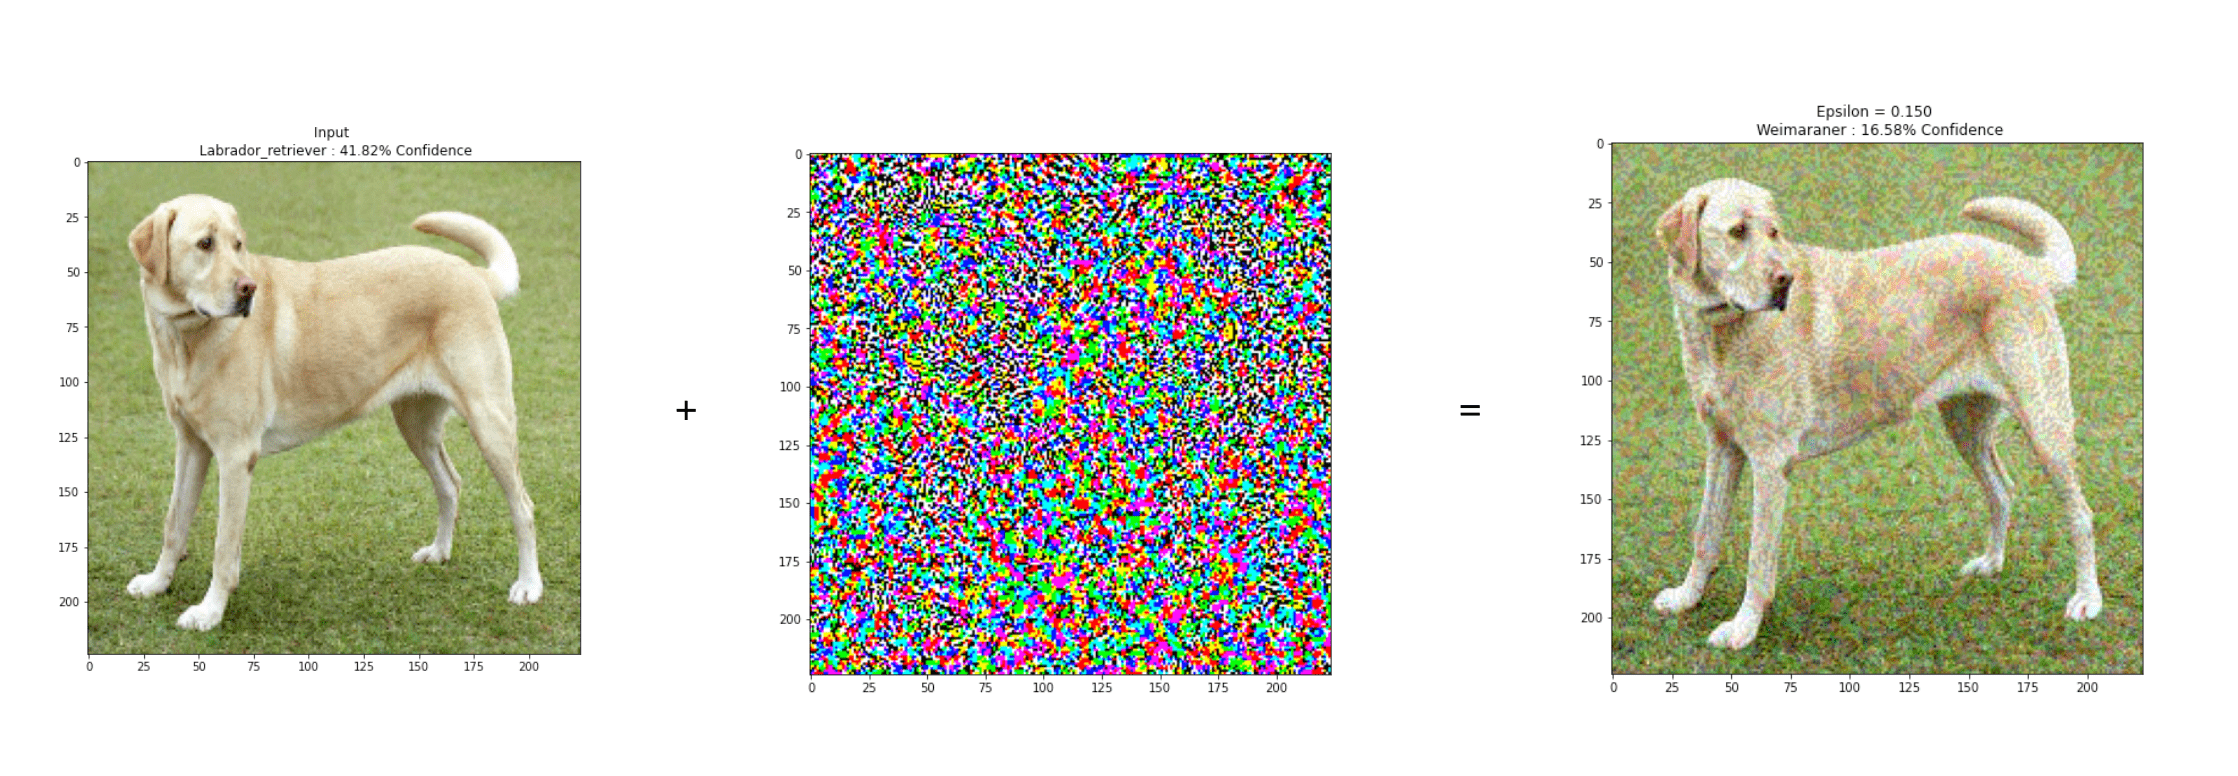
\includegraphics[width = \textwidth]{{fig/adv_example.png}}
    \caption{An example of adversarial pertubation resulting successful adversarial attack}
    \label{adv_example}
\end{figure}

One explaination\cite{cite:ytb_talk} of why adversarial attack works is because there is a natural distinction between how we read and how machine read into a piece of information. When we human are asked to classify between a \textit{dog} from a \textit{cat}, we know to focus on the ears and snout:


\begin{figure}[H]
    \centering
    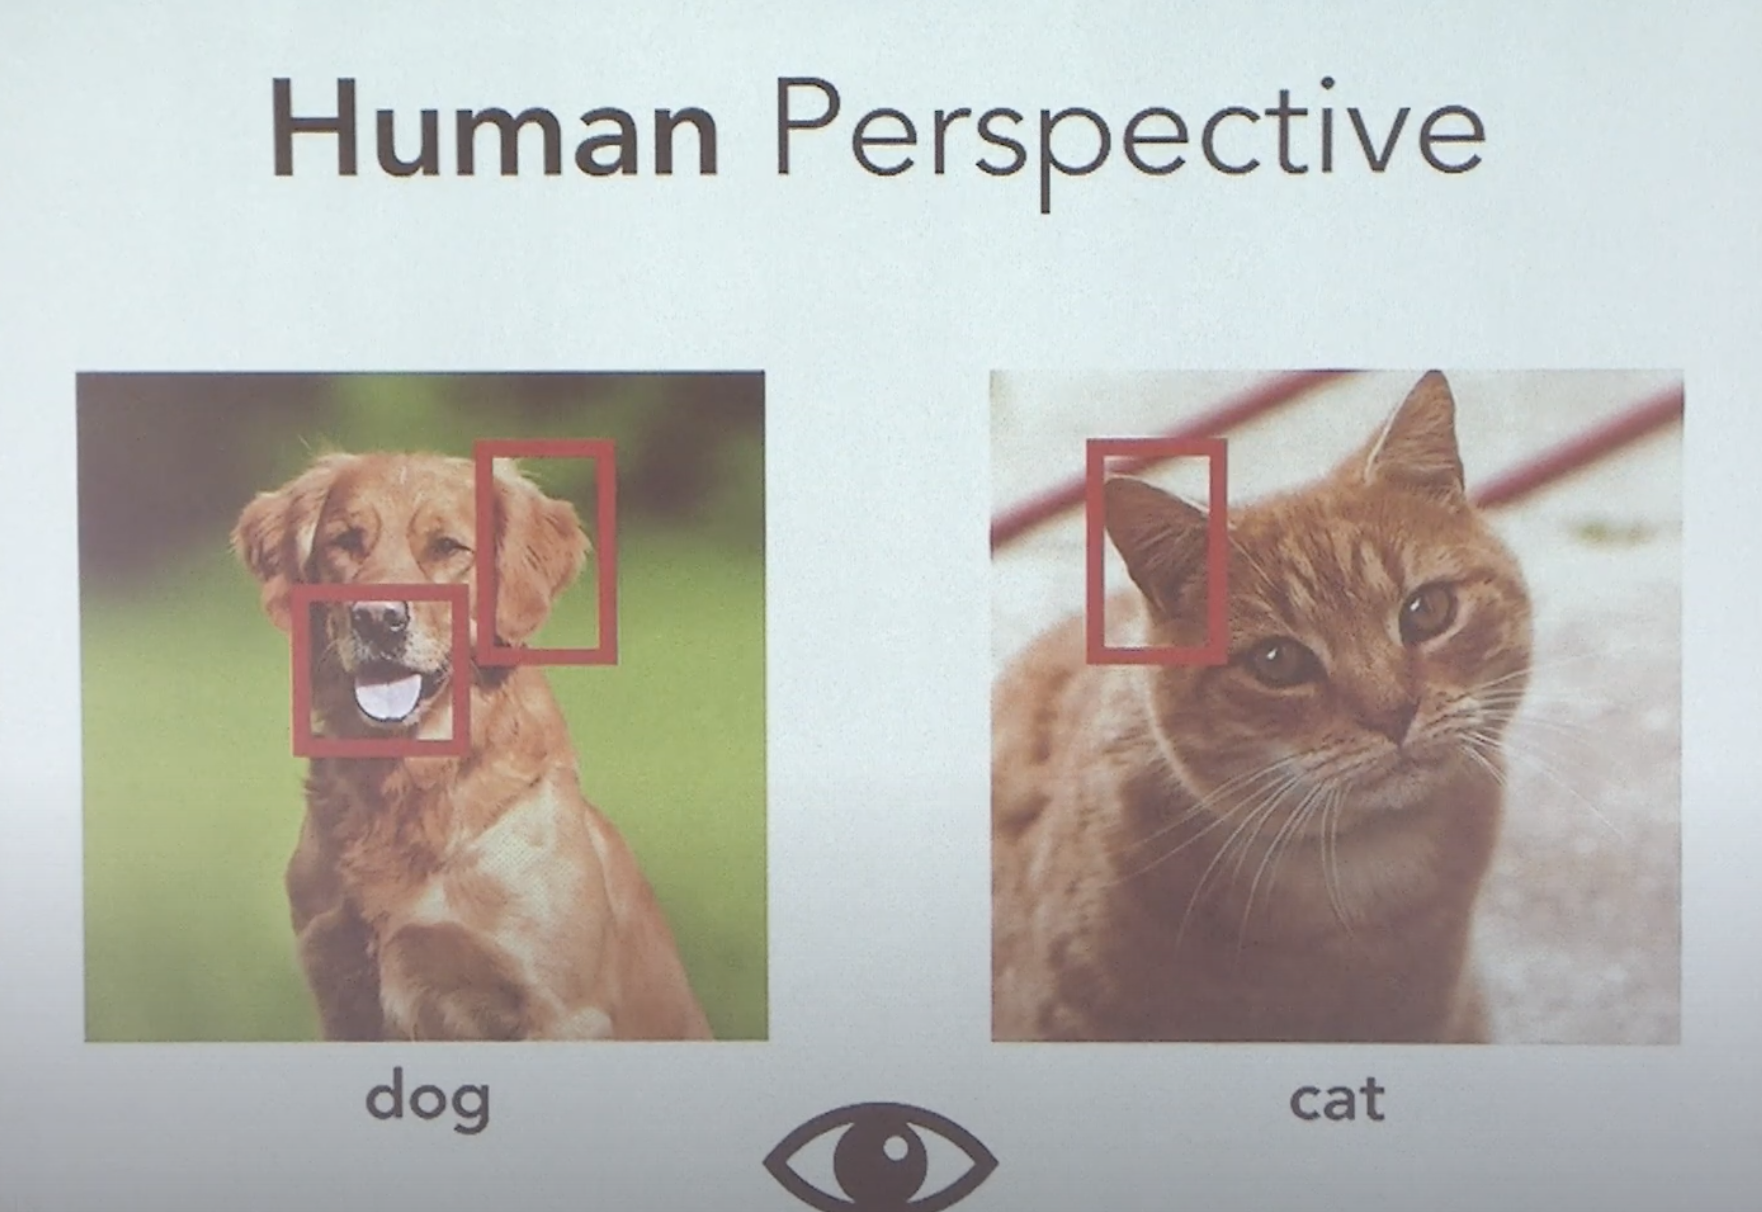
\includegraphics[width = 0.6\textwidth]{{fig/ytb_human.png}}
    \caption{Human perspective}
    \label{ytb_human}
\end{figure}

and we considered the pertubation in [\figurename{\ \ref{adv_example}}] to be meaningless because we cannot digest useful information out of it. But that might not be the case to the ``eyes'' of a machine as it has no knowledge about cats and dogs. To ``translate'' the machine's perspective to ``human terms,'' how machine look at these cat/dig pictures are probably like the following:

\begin{figure}[H]
    \centering
    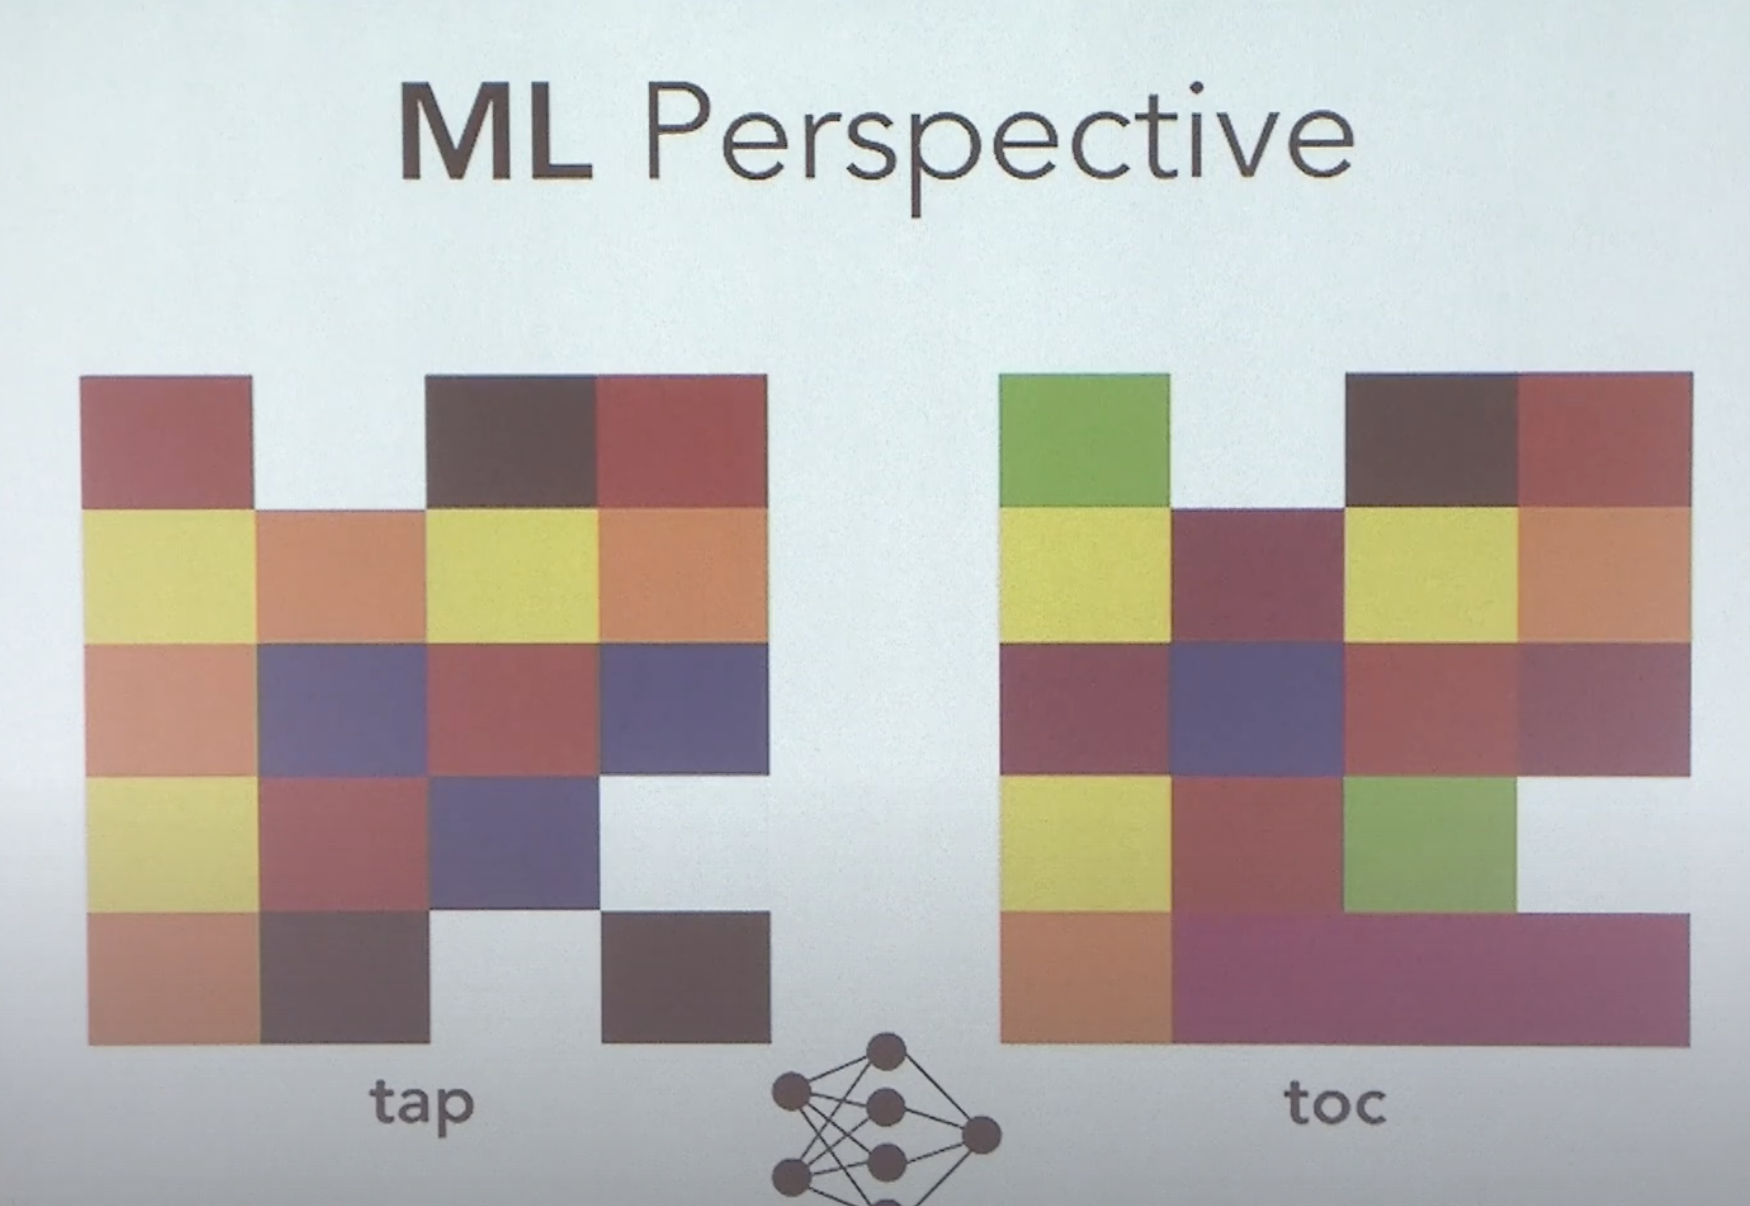
\includegraphics[width = 0.6\textwidth]{{fig/ytb_machine.png}}
    \caption{Machine perspective}
    \label{ytb_machine}
\end{figure}

In fact, a machine might considers the pertubation in [\figurename{\ \ref{adv_example}}] to be more ``informative'' than the features we care about (ears and snout). And since models are set to maximize accuracy as a general goal, it will utilize both features -- both the \textit{robust features} (features that keep being robust after adversarial pertubation), and the \textit{non-robust features} (e.g., some ``noise'' to human):

\begin{figure}[H]
    \centering
    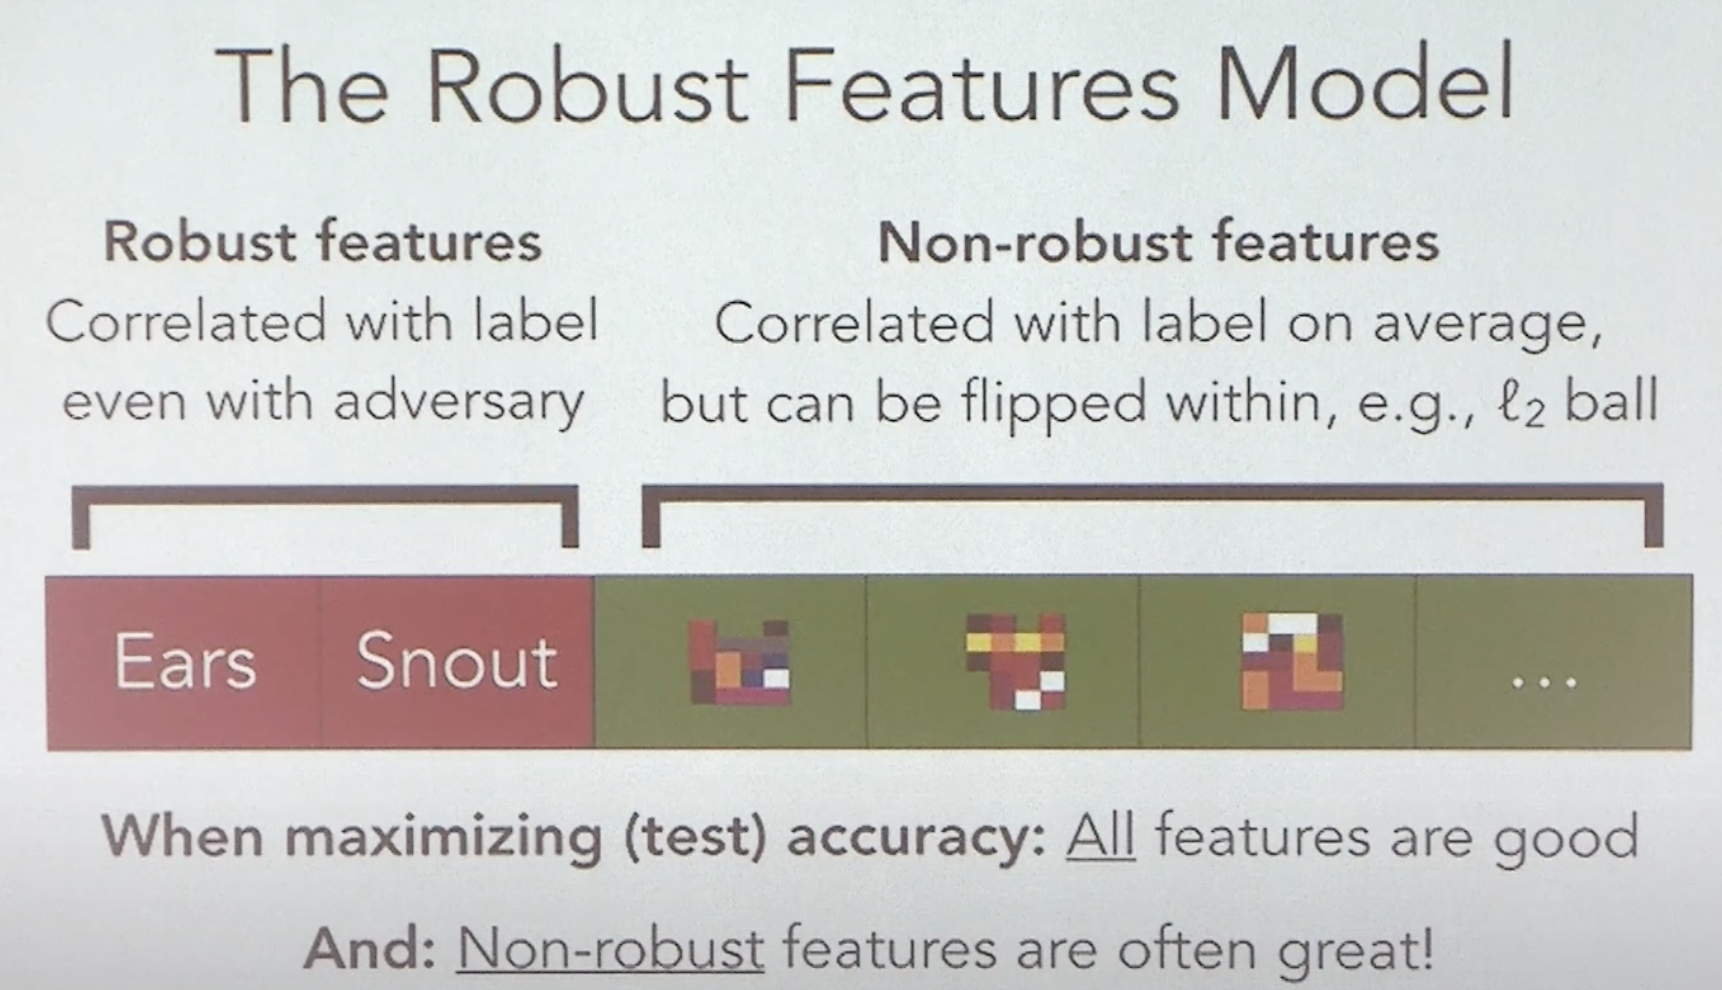
\includegraphics[width = 0.6\textwidth]{{fig/ytb_features.png}}
    \caption{Robust and non-robust features}
    \label{ytb_features}
\end{figure}

Thus, if a model's decision is largly base on these non-robust features, we may apply adversarial pertubations to adjust these features and causing the model to output false results. \newline

For this paper in particular, we will look into \textit{evasion attack} (causing the model to output false result by modifying the input), \textit{poisoning attack} (alter the training set of a model to make it produce inaccruate decision boundaries), and some corresponding defense methods against these attacks.


\section{Individual Reports}

\subsection{Shaochen (Henry) Zhong's Individual Report}
\subsubsection{Overview}

I have wholeheartedly lead and contributed to this group project, below is an itemized list of my contributions. I have inquired Dr. Ray and confirmed these can be considered as ``extra works'' and maybe give me some grade boost. Thanks :)
\begin{itemize}
    \item Read 3 papers on algorithms.
    \item Implemented 2 algorithms (\ilc{FGSM} and \ilc{Hop Skip Jump}) with 3 extensions.
    \item Piplined attack algorithms to work with 2 datasets, collected almost all (7 algorithms/useable extensions) attack experiments data (except \ilc{backdoor} and \ilc{one pixel attack}) for the comparative evaluations.
    \item Piplined and collected experiments data for \ilc{FGSM, Hop Skip Jump, DeepFool} attacks (and their useable extensions) against \ilc{Detector} and \ilc{Spatial Smoothing} defenses on 2 datasets.
    \item Implemented $L_2$ and $L_{\infty}$ \textit{perturbation budget} to aid comparative evaluation.
    \item Wrote \textbf{Introduction and Significance} section.
    \item Plotted all graphs and charts in \textbf{Comparative Study and Discussion}.
    \item Helped group move forward by making technical decisions, distributing works, setting up deadlines, and facilitating coordination between groupmates.
\end{itemize}

\subsubsection{\ilc{Fast Gradient Sign Method}}
\paragraph{Algorithm Intuition}

\ilc{FGSM}\cite{cite:fsgm_paper} is a \textit{white-box} evasion attack algorithm. Being \text{white-box} means the attacker is assumed to have access to the internal of the model: the structure, the parameters... basically each and every details of the model is considered to be known.

In this case, we mostly care about the \ilc{loss} function of the model. The intuition of \ilc{FGSM} is elegent and effective -- in short: gradient ascent. Assume we have an benign example $x$ with label $y$, and we are trying to make it adversarial by letting the model classify $x_{\text{adv}}$ to be not $y$. We apply the following pertubation on $x$ to achieve an $x_{\text{adv}}$

\begin{equation}
    x_{\text{adv}} = x + \epsilon \cdot \text{sign}(\nabla_x J(\theta, x, y))
    \label{fgsm_eq}
\end{equation}

where $J$ is the \ilc{loss} function and $\theta$ is the parameters of the model. It is clearly to tell that by finding a proper amount of $\epsilon$, we know $x_{\text{adv}}$ will eventually cross the $y$ and $\neg y$ decision boundary and be classified as a $\neg y$ object. We know this direction will lead to a $\neg y$ space because a model is designed to minimize the \ilc{loss} -- thus it is always doing gradient descent -- and by going against the gradient to do gradient ascent, it will ``maximize'' the \ilc{loss} and eventually be misclassified. And if the value of $\epsilon$ is small enough, the $x_{\text{adv}}$ will sill perserve enough semantic from $x$ and thus relatively indistinguishable to human eyes. Like the following exmaple in [\figurename{\ \ref{google_panda}}]:


\begin{figure}[H]
    \centering
    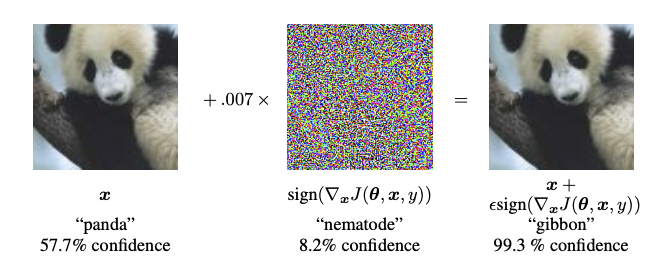
\includegraphics[width = 0.8\textwidth]{{fig/google_panda.png}}
    \caption{Applying gradient ascent pertubation to a panda image, $\epsilon = 0.07$}
    \label{google_panda}
\end{figure}

Although the $x_{\text{adv}}$ on the RHS has been adversarially altered, because the distance of pertubation is small enough, it sill looks like a panda -- a.k.a. perserving the majority semantic of $x$.

\subparagraph{Extension 1: \ilc{Targeted Fast Gradient Sign Method}}

As standard \ilc{FGSM}, assuming implemented on $x$ with $y$-label, only cares about reaching a space of $\neg y$. This can be undesired for certain application. One scenario maybe is to attack the OCR system of bank checks (which is usually the goal when attacking \textit{MINIST}), the attacker would want a lower valued number to be recognized as a higher valued number (e.g., \ilc{0 -> 9}), but not vice versa. Thus, I have implemented a targeted version of \ilc{FGSM}, where instead of doing gradient ascent to $y$ like in [Equation \ref{fgsm_eq}], it does gradient descent towards the label of desired target.\newline

Say we have a target of $x_t$ with label $y_t$, the mathematical intuition of \ilc{T-FGSM} is:

\begin{equation}
    x_{\text{adv}} = x - \epsilon \cdot \text{sign}(\nabla_x J(\theta, x, y_t))
    \label{t_fgsm_eq}
\end{equation}

Note we are back to standard gradient descent like running a normal model. This is because we want to minimize the \ilc{loss} of $x_{\text{adv}}$ with label $y_t$ -- which is not guaranteed by randoming doing gradient ascent out of $y$ as that might not be the right direction.

\subparagraph{Extension 2: \ilc{Iterative Fast Gradient Sign Method}}

One major drawback of traditional \ilc{FGSM} is to decide the $\epsilon$ value in [Equation \ref{fgsm_eq}]. Intuitively, such $\epsilon$ can't be too small, otherwise the applied pertubation will be too small to make $x_{\text{adv}}$ across the $y$ to $\neg y$ decision boundary. However, it also can't be too large as it will lose the semantic of $x$, like in the follwing example we applied an $\epsilon = 30$ to the Labrador Retriever in [\figurename{\ \ref{adv_example}}] and this is just pure noise:

\begin{figure}[H]
    \centering
    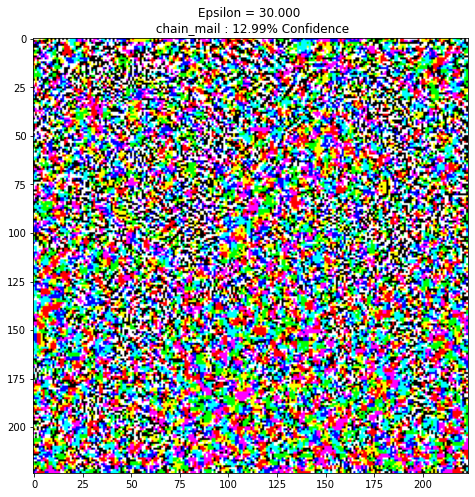
\includegraphics[width = 0.2\textwidth]{{fig/google_fgsm_overshoot.png}}
    \caption{Perturbed Labrador Retriever with $\epsilon = 30$}
    \label{google_fgsm_overshoot}
\end{figure}

In this case, although [\figurename{\ \ref{google_fgsm_overshoot}}] is still an successful adversarial attack to the machine (as it was classified as \textit{Chain Mail} for some reasons). The attack is by essence meaningless as it has lost all semantics of a Labrador Retriever -- and we might as well just swap it with an actual chain mail picture and call it a successful attack.\newline

\noindent More important, depending on the decision boundaries of a model, some value of $\epsilon$, altough being large enough, might also fail the attack. Consider a model with the following decision boundary:

\begin{figure}[H]
    \centering
    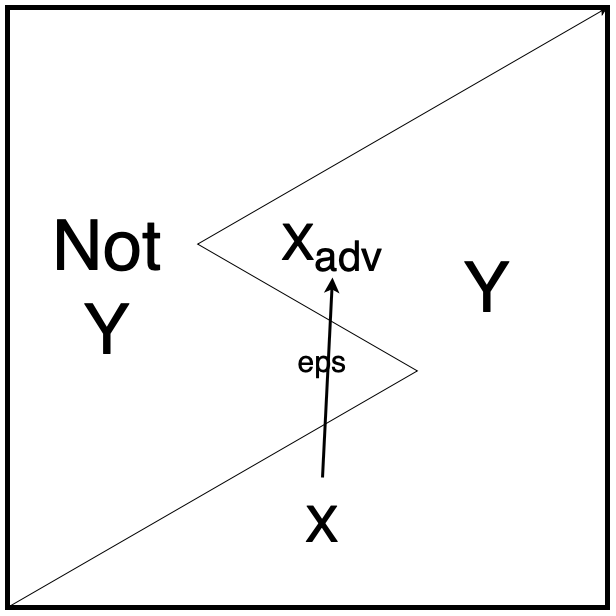
\includegraphics[width = 0.3\textwidth]{{fig/overshoot_non_target.png}}
    \caption{Potential $\epsilon$ overshoot}
    \label{overshoot_non_target}
\end{figure}

As demoed in [\figurename{\ \ref{google_fgsm_overshoot}}], with an unfortunate $\epsilon$, even being large, an attack can still fail. Thus I took advantage of doing a \textit{white-box} attack and implemented an iterative version of \ilc{FGSM}. As instead of taking an \textit{one-shot} pertubation, it takes one and another small pertubations to reach to a decision boundary; once the prediction is changed, it stops applying further pertubations.

The mathematical intuition of this algorithm will be like [Equation \ref{i_fgsm_eq}]

\begin{equation}
    x_{\text{adv}_{i+1}} = x_{\text{adv}_{i}} + \epsilon_{\text{step}} \cdot \text{sign}(\nabla_x J(\theta, x_{\text{adv}_{i}}, y))
    \label{i_fgsm_eq}
\end{equation}

where $\epsilon_{\text{step}} \ll \epsilon$, and we can hard bound the accumulation of $\epsilon_{\text{step}}$ to be less or equal to $\epsilon$ so the algorithm try to perturb an example which is far away from its decision boundary and running forever. And since the final $x_{\text{adv}} $ will be right on the decision boundary (granted a small enough $\epsilon_{\text{step}}$ was used), it will perserve a healthy amount of semantics of $x$.

\subparagraph{Extension 3: \ilc{Iterative Targeted Fast Gradient Sign Method}}

Naturally, I combined my two implementation together. [Equation \ref{it_fgsm_eq}] is the mathematical intuition of the algorithm:

\begin{equation}
    x_{\text{adv}_{i+1}} = x_{\text{adv}_{i}} - \epsilon_{\text{step}} \cdot \text{sign}(\nabla_x J(\theta, x_{\text{adv}_{i}}, y_t))
    \label{it_fgsm_eq}
\end{equation}

\paragraph{Algorithm Implementation}

I implemented \ilc{FGSM} and its three extentions with the help of \ilc{ART}\cite{cite:art}. It is a \ilc{Python}-based open-source libarary that taken care of the engineering aspects of adversarial machine learning testing. Specifically, I used \ilc{ART}'s \ilc{KerasClassifier} to wrap around a pretrained model of \textit{MINIST} and \textit{CIFAR-10} as my victim model -- I can do this because all my implemented algorithms and extensions is attacking a trained model, so how the model was trained is not in my interest of evaluation.\newline

I first gather the \ilc{x\_test} sample set from my dataset, then I feed into the pretained model to get \textit{benign acc} reading. Then I apply the below actiovation methods (by choice)

\begin{lstlisting}
attacker = FastGradientSignMethod(classifier, eps=0.3, batch_size = 32)
x_test_adv = attacker.generate(x_test[:num]) # non-targeted
x_test_adv = attacker.generate_targeted(x_test[:num], x_test[0]) # targeted
x_test_adv = attacker.generate_iterative(x_test[:num]) # iterative non-targeted
x_test_adv = attacker.generate_targeted_iterative(x_test[:num], x_test[0]) # iterative targeted
\end{lstlisting}

to generate the adversarially perturbed \ilc{x\_test\_adv} from \ilc{x\_test}. I then feed \ilc{x\_test\_adv} into the pretained model and collect the \textit{adversarial acc} reading.

In the meantime, I collect $L_2$ and $L_\infty$ distances between a benign and an adversarial images (calculated by channel) to be a mertrics of quantifying \textit{pertubation budget}. I also implemented a runtime counter to register how long it took an attack method to run -- you may see them in my following Section \ref{fgsm_exp} and comparative study sections like \ref{attack_algo}.

\paragraph{Experiments and Evaluation}\label{fgsm_exp}

Since I have implemented multiple extensions and \ilc{FGSM} have several params to tone with, I have did a vast amount of experiments. We later decided to go with \ilc{eps = 0.3, eps\_step = 0.05}


\begin{figure}[H]
    \centering
    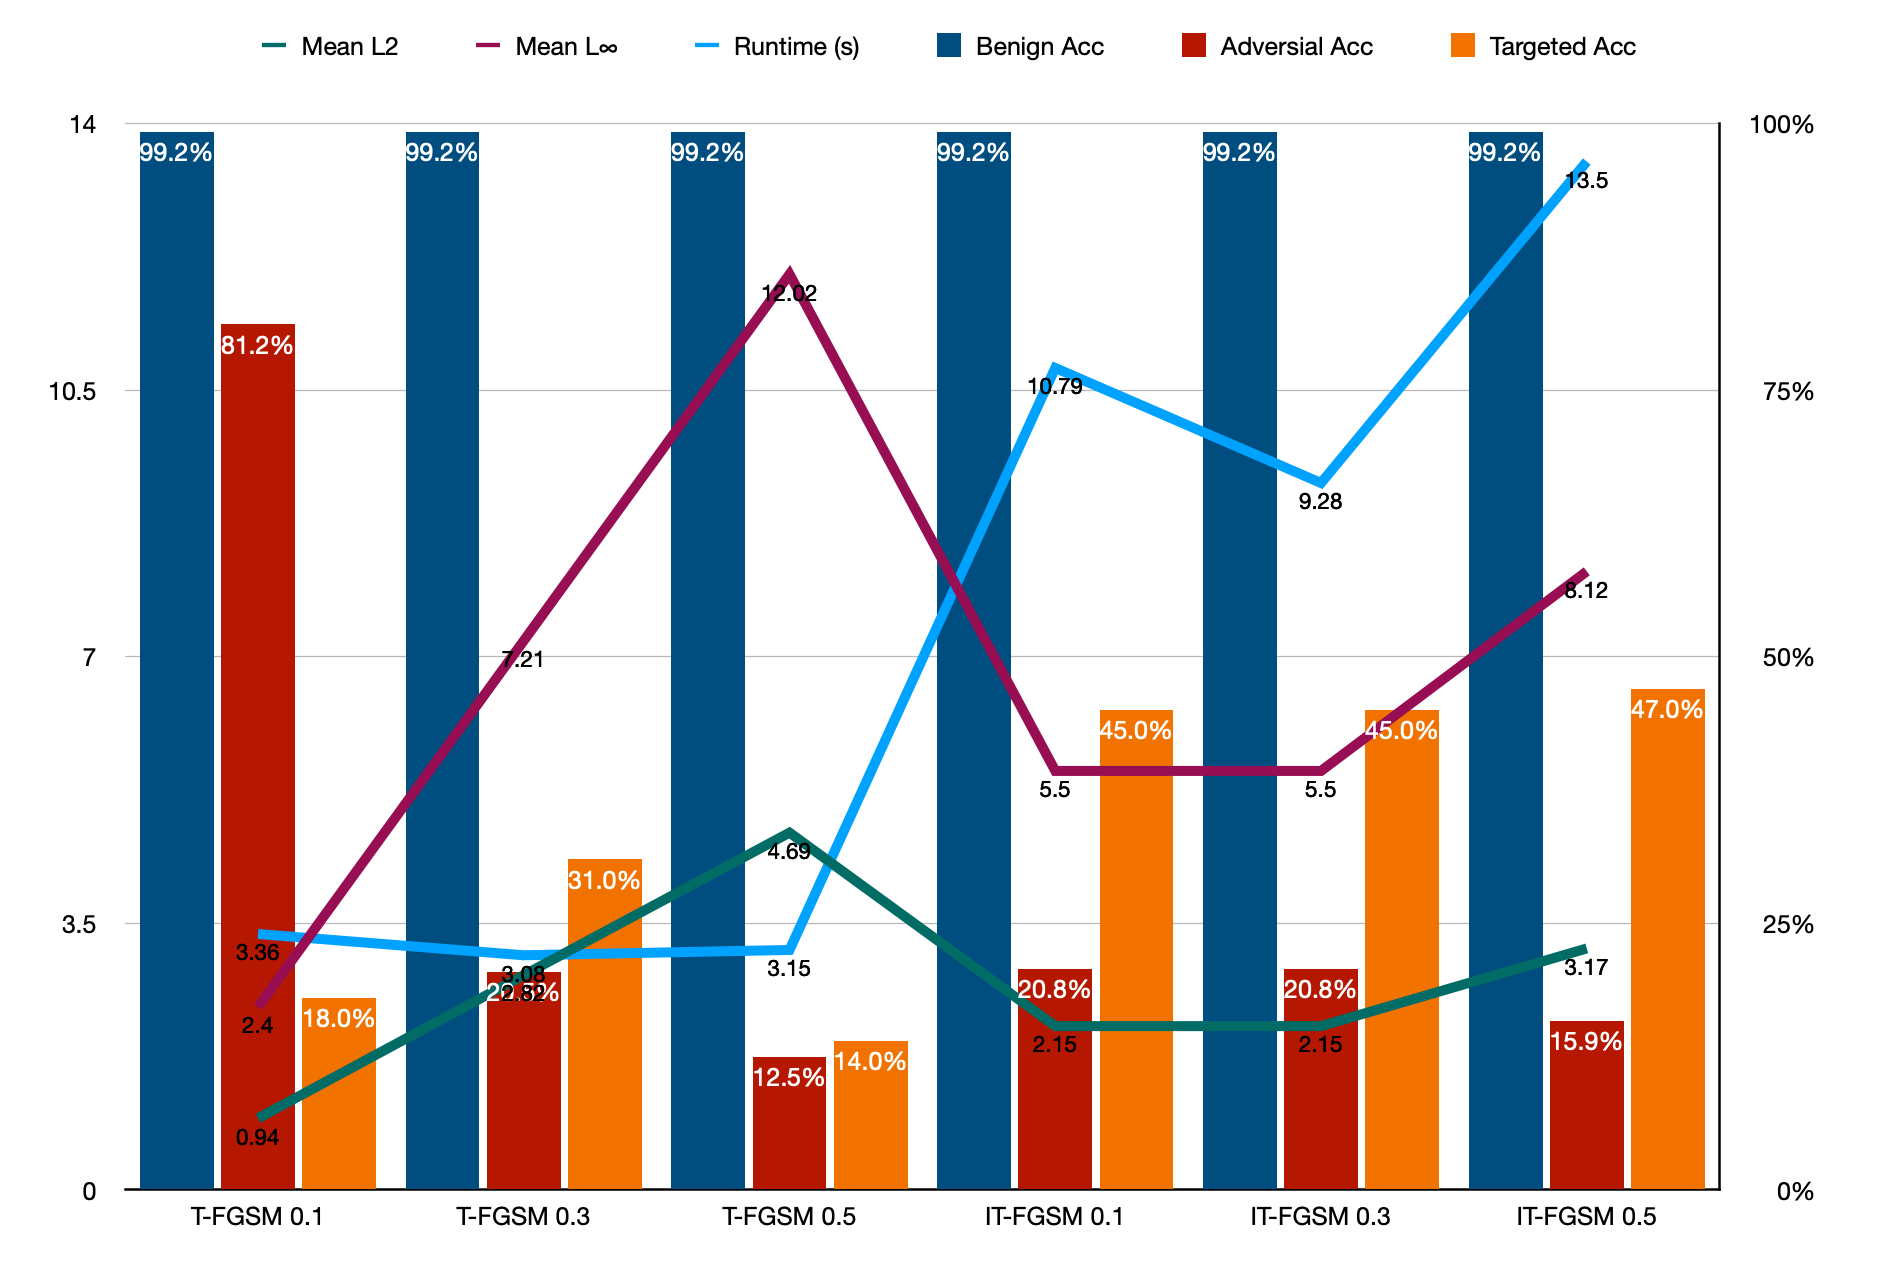
\includegraphics[width = 1\textwidth]{{fig/i_fgsm_minist.png}}
    \caption{\ilc{T-FGSM} and \ilc{IT-FGSM} with $\epsilon = \{ 0.1, 0.3, 0.5\}$ on \textit{MINIST}}
    \label{i_fgsm_minist}
\end{figure}

because in [\figurename{\ \ref{google_fgsm_overshoot}}], we may observe the mentioned ``overshooting'' problem as in \ilc{T-FGSM} the \textit{Targeted Acc} is decreasing with $\epsilon$ increasing. However, this is sloved by implementing \ilc{IT-FGSM}, the \textit{Targeted Acc} is growing with the $\epsilon$.

Also we noticed we ended with a much better \textit{pertubation budget} in \ilc{IT-FGSM}. This is because the algorithm stop pertubation once it reached the target label, thus remain a smaller and therefore preferred $L_2$ and $L_\infty$. But we do realize even in \ilc{IT-FGSM}, the $L_2$ and $L_\infty$ is increasing with $\epsilon = 0.3 \rightarrow 0.5$, this is because with a bigger $\epsilon$ the algorithm is trying to move picture that are relatively far away from the target to be the target -- this is undesired the resulted images will likely losing semantics, and it cost more computing power to do so (which is also reflected by the \textit{runtime} data, as it is significantly slower in $\epsilon = 0.5$ than $\epsilon = 0.3$). Thus, we set the this to be the parameters of \ilc{FGSM}-related algorithms in comparative studies.



\subsubsection{\ilc{Hop Skip Jump}}

\ilc{HSJ}\cite{cite:hsj_paper} is another evasion attack algorithm I implemented.

\paragraph{Algorithm Intuition}
\paragraph{Algorithm Implementation}
\paragraph{Experiments and Evaluation}


\subsubsection{\ilc{Feature Collision}}
\paragraph{Algorithm Intuition}


\subsection{Minyang Tie's Individual Report}


\subsection{Alex Useloff's Individual Report}


\subsection{Austin Keppers' Individual Report}
\subfile{individual_reports/agk51}

\subsection{David Meshnick's Individual Report}

\section{Comparative Study and Discussion}

In this section, we will present a comparative study between some algorithms (and their comparable extensions) we implemented.

\subsection{Overview}

\subsubsection{Datasets and Sample Selections}

For the tesing datasets, we opted to use \textit{MINIST} \cite{cite:minist} and \textit{CIFAR-10} \cite{cite:cifar10}. In short, \textit{MINIST} is a database of handwritten digits and \textit{CIFAR-10} is a database for tiny images, as demonstrated below in  [\figurename{\ \ref{MINIST}}] and [\figurename{\ \ref{CIFAR}}].


\begin{figure}[H]
\minipage{0.4\textwidth}
    \centering
    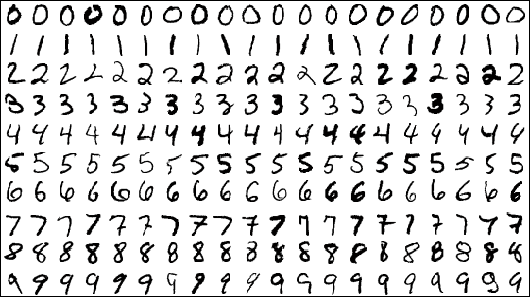
\includegraphics[width = \textwidth]{{fig/MINIST.png}}
    \caption{An selection of \textit{MINIST} database}
    \label{MINIST}
\endminipage\hfill
\minipage{0.4\textwidth}
    \centering
    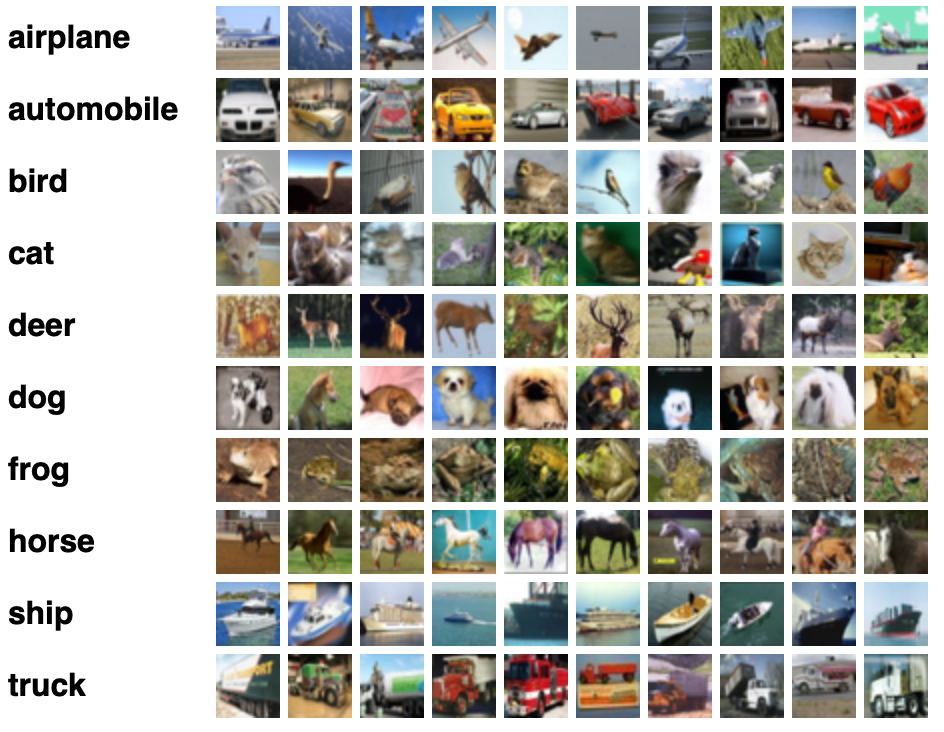
\includegraphics[width =\textwidth]{{fig/CIFAR10.png}}
    \caption{An selection of \textit{CIFAR-10} database}
    \label{CIFAR}
\endminipage
\end{figure}

\noindent Our decision of using these two datasets are base on the consideration of:
\begin{itemize}
    \item Both datasets are pre-labeled and have pretrained model available for use. So we may save time on training the victim model(s), and also have some consistent baselines to refer to.
    \item Both datasets are lightweight in terms of image resolutions, so when evaluating computational-heavy algorithms (e.g. \ilc{Hope Skip Jump}), we are able to get the experiments data either locally or with minimum use of cloud services.
    \item Having ORC and image classifying tasks (in general) together can be a very fair coverage of the actual applications of adversarial learning.
    \item \textit{MINIST} specifically has a close-to-pure background color, which is a great for human to evaluate as sometime the perturbation on a colorful picture can be unnoticeable to human eyes.
    \item The toolbox of choice \textit{adversarial-robustness-toolbox} a.k.a \ilc{ART} have wrapper methods around these two models, and can load their pretained models as \ilc{ART}'s victim classifiers (we have specifically inquired Dr. Ray that it is ok to \ilc{import} this kind of facilities).
\end{itemize}

We have thought about using a third database like \textit{ImageNet} or \textit{IRIS}, but with the combinations of attacks and defenses algorithms we already have a very heavy experiments workload. So we opted to only use these two. However, considered the image quality of \textit{MINIST} and \textit{CIFAR-10} are rather on the low side, we used some \textit{ImageNet} images to demo our work and concepts.

\subsubsection{ART}

\textit{adversarial-robustness-toolbox}\cite{cite:art} a.k.a \ilc{ART} is an IBM-sponsered library that provides tools for necessary adversarial learning experiments. We have utlized \ilc{ART}'s facilities on loading dataset, wrapping victim classifiers, and piplining attack and defense algorithms together. We cannot finish this project without this library, so much credit to them.

\subsubsection{Metrics}

As we are not doing binary classifications, \textit{accuracy} will be our top piority. This is also the case for general goal of adversarial learning, as we either what to attack the model to lower its \textit{accuracy}, or we want to defend from an attack with increased robustness -- thus higher  \textit{accuracy}.\newline

\noindent However, another important aspect of adversarial learning is, in most of the cases, we want the our attack image to be only ``adversarial'' to a computer model, but not to human eyes. This is first because without such restraint we may simply swap a dog picture with a cat picture and call it a successful attack, which will make the task meaningless. Second, it is because for most of the time we want our attack to be ``stealthy'' -- and a collection of pixels noises is simply not so much of that.

\begin{figure}[H]
\minipage{0.25\textwidth}
    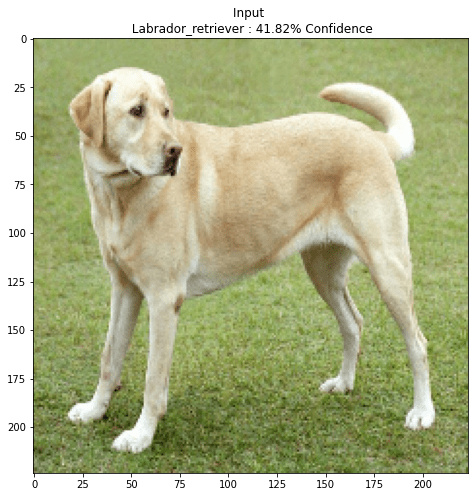
\includegraphics[width = \textwidth]{{fig/google_fgsm_1.png}}
\endminipage\hfill
\minipage{0.25\textwidth}
    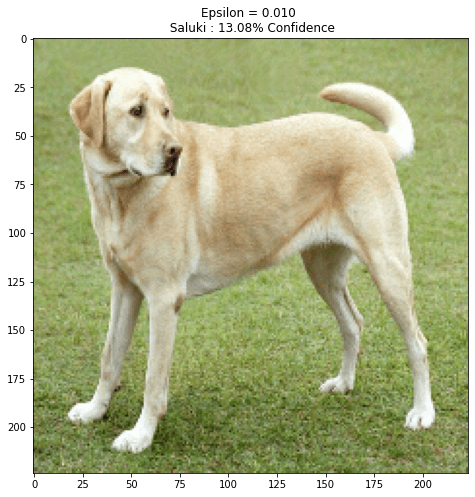
\includegraphics[width = \textwidth]{{fig/google_fgsm_2.png}}
\endminipage\hfill
\minipage{0.25\textwidth}
    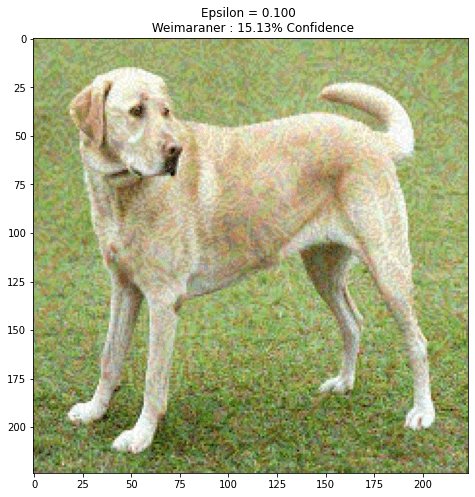
\includegraphics[width = \textwidth]{{fig/google_fgsm_3.png}}
\endminipage\hfill
\minipage{0.25\textwidth}
    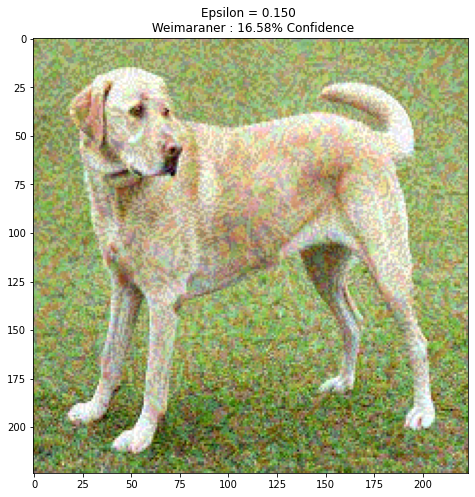
\includegraphics[width = \textwidth]{{fig/google_fgsm_4.png}}
\endminipage
\caption{A Labrador Retriver with different levels of perturbations}
\label{fgsm_dog}
\end{figure}

Thus, keeping the ``semantic'' of the original image is important in terms of making adversarial examples. However we must have a way to quantify such perturbations -- as it can be very hard to tell like shown in [\figurename{\ \ref{fgsm_dog}}] \cite{cite:google_fgsm} -- so that we can numerically conclude and justify the claim if a image has lost it semantic (and by how much).

The metrics we found is \textit{perturbation budget}\cite{cite:perb_budget}, it defined as:

\begin{equation}
     \epsilon = || x_{\text{adv}} - x ||
     \label{perb_budget_equation}
\end{equation}

where $epsilon$ in [Equation \ \ref{perb_budget_equation}] is the \textit{perturbation budget}. However, we have different choices on calculating the distance metrics. In this case, we opted to use $L_2$ and $L_{\infty}$ as they represent the \textsc{Euclid} distance and maximum magnitude between pixels -- which covered the perturbation of a picture both holistically and ``extremely.''

Specifically in practice, we calcualte the $L_2$ and $L_{\infty}$ of two images channel by channel then add them together. The principle is we will want the these numbers to be as small as possible, as long as the adversarial image we created still have an adversarial affect to a model. Note if an algorithm is iterative, a smaller \textit{perturbation budget} also means smaller computation cost -- as less iteration were done.\newline

\noindent Another thing that maybe worth mentioning is since we used pretained victim model, we didn't do anything like N-fold cross validation as we are seeking effects out of a trained model, but not to train one (maybe except \ilc{Neural Cleanse} as it does retain the model). But we do average our trials to make sure our experiment results are reproducable.


\subsubsection{Adversarial Rivalry}

We have implemented and experimented multiple attack and defense algorithms, but not all of them can be compared together due to various reasons. In our cases, we opted to not to have some algorithms compared together, or even not to include some algorithm in our comparative study.

We opted to compare \ilc{Fast Gradient Sign Method} (non-targeted, with one-shot and iterative implementions), \ilc{Hop Skip Jump}, \ilc{DeepFool} (and \ilc{Dynamic DeepFool} -- an extension implemented by David) together as they are all the non-targed evasion algorithm we implemented. We opted to not include \ilc{Backdoor} in this set of comparsion as it evasion attacks were done in the assumption of having a trained model, it doesn't make sense to have posioning -- which can alter the training set of a model -- to be part of the comparsion. Similarily, the two targeted extensions \ilc{FGSM} is excluded from this comparsion as in this context it is the magnitude of decrease of model \textit{accuracy} in general we care about, but not which exact label the model most classifies to.

Likewise, we opted to not compare any other algorithm except \ilc{Backdoor} to against \ilc{Neural Cleanse}, as: Minyang please input here.

Also we are not comparing different defense algorithms against a same attack algorithm. This is not because we are not interested in the performance difference between defense algorithm. It is simply because we have already elimited \ilc{Neural Cleanse} due to its retrain nature; and for the other two remained defense algorithm \ilc{Binary Input Detector} and \ilc{Spatial Smoothing}, the former one is designed to recognize and flag an adversarial image, where the latter is to increase model robustness so that it can better classified adversarially perturbed images -- so they can't be compared.


\subsection{Attack Algorithms}\label{attack_algo}

Note \ilc{I-FGSM} represents (non-targted, one-shot) \ilc{Iterative Fast Gradient Sign Method};  \ilc{D-DeepFool} represents \ilc{Dynamic DeepFool}. The \ilc{FGSM} is running with params being \ilc{batch\_size = 32, eps = 3}, and the \ilc{I-FGSM} is running on the same setting with \ilc{eps\_step = 0.05} as we have found in Henry's individual report with \ilc{eps\_step > 0.05} we might ``overshot'' ourself. \newline

\ilc{Hop Skip Jump} a.k.a. \ilc{HSJ} is a very computational-heavy algorithm. When possible, we will use \ilc{max\_iter=64, max\_eval=1000, init\_eval=100} which is close to the authors suggested setting (except the authors suggests \ilc{max\_eval = 100000} which is impossible to replicate with our resource). But often time we are limited for \ilc{max\_iter=8, max\_eval=100, init\_eval=10}. \newline

Unless specifically addressed, the base line model is a the pretrained model of dataset wrapped in \ilc{ART}'s \ilc{KerasClassifier}.

\subsubsection{Evasion}


\begin{figure}[H]
    \centering
    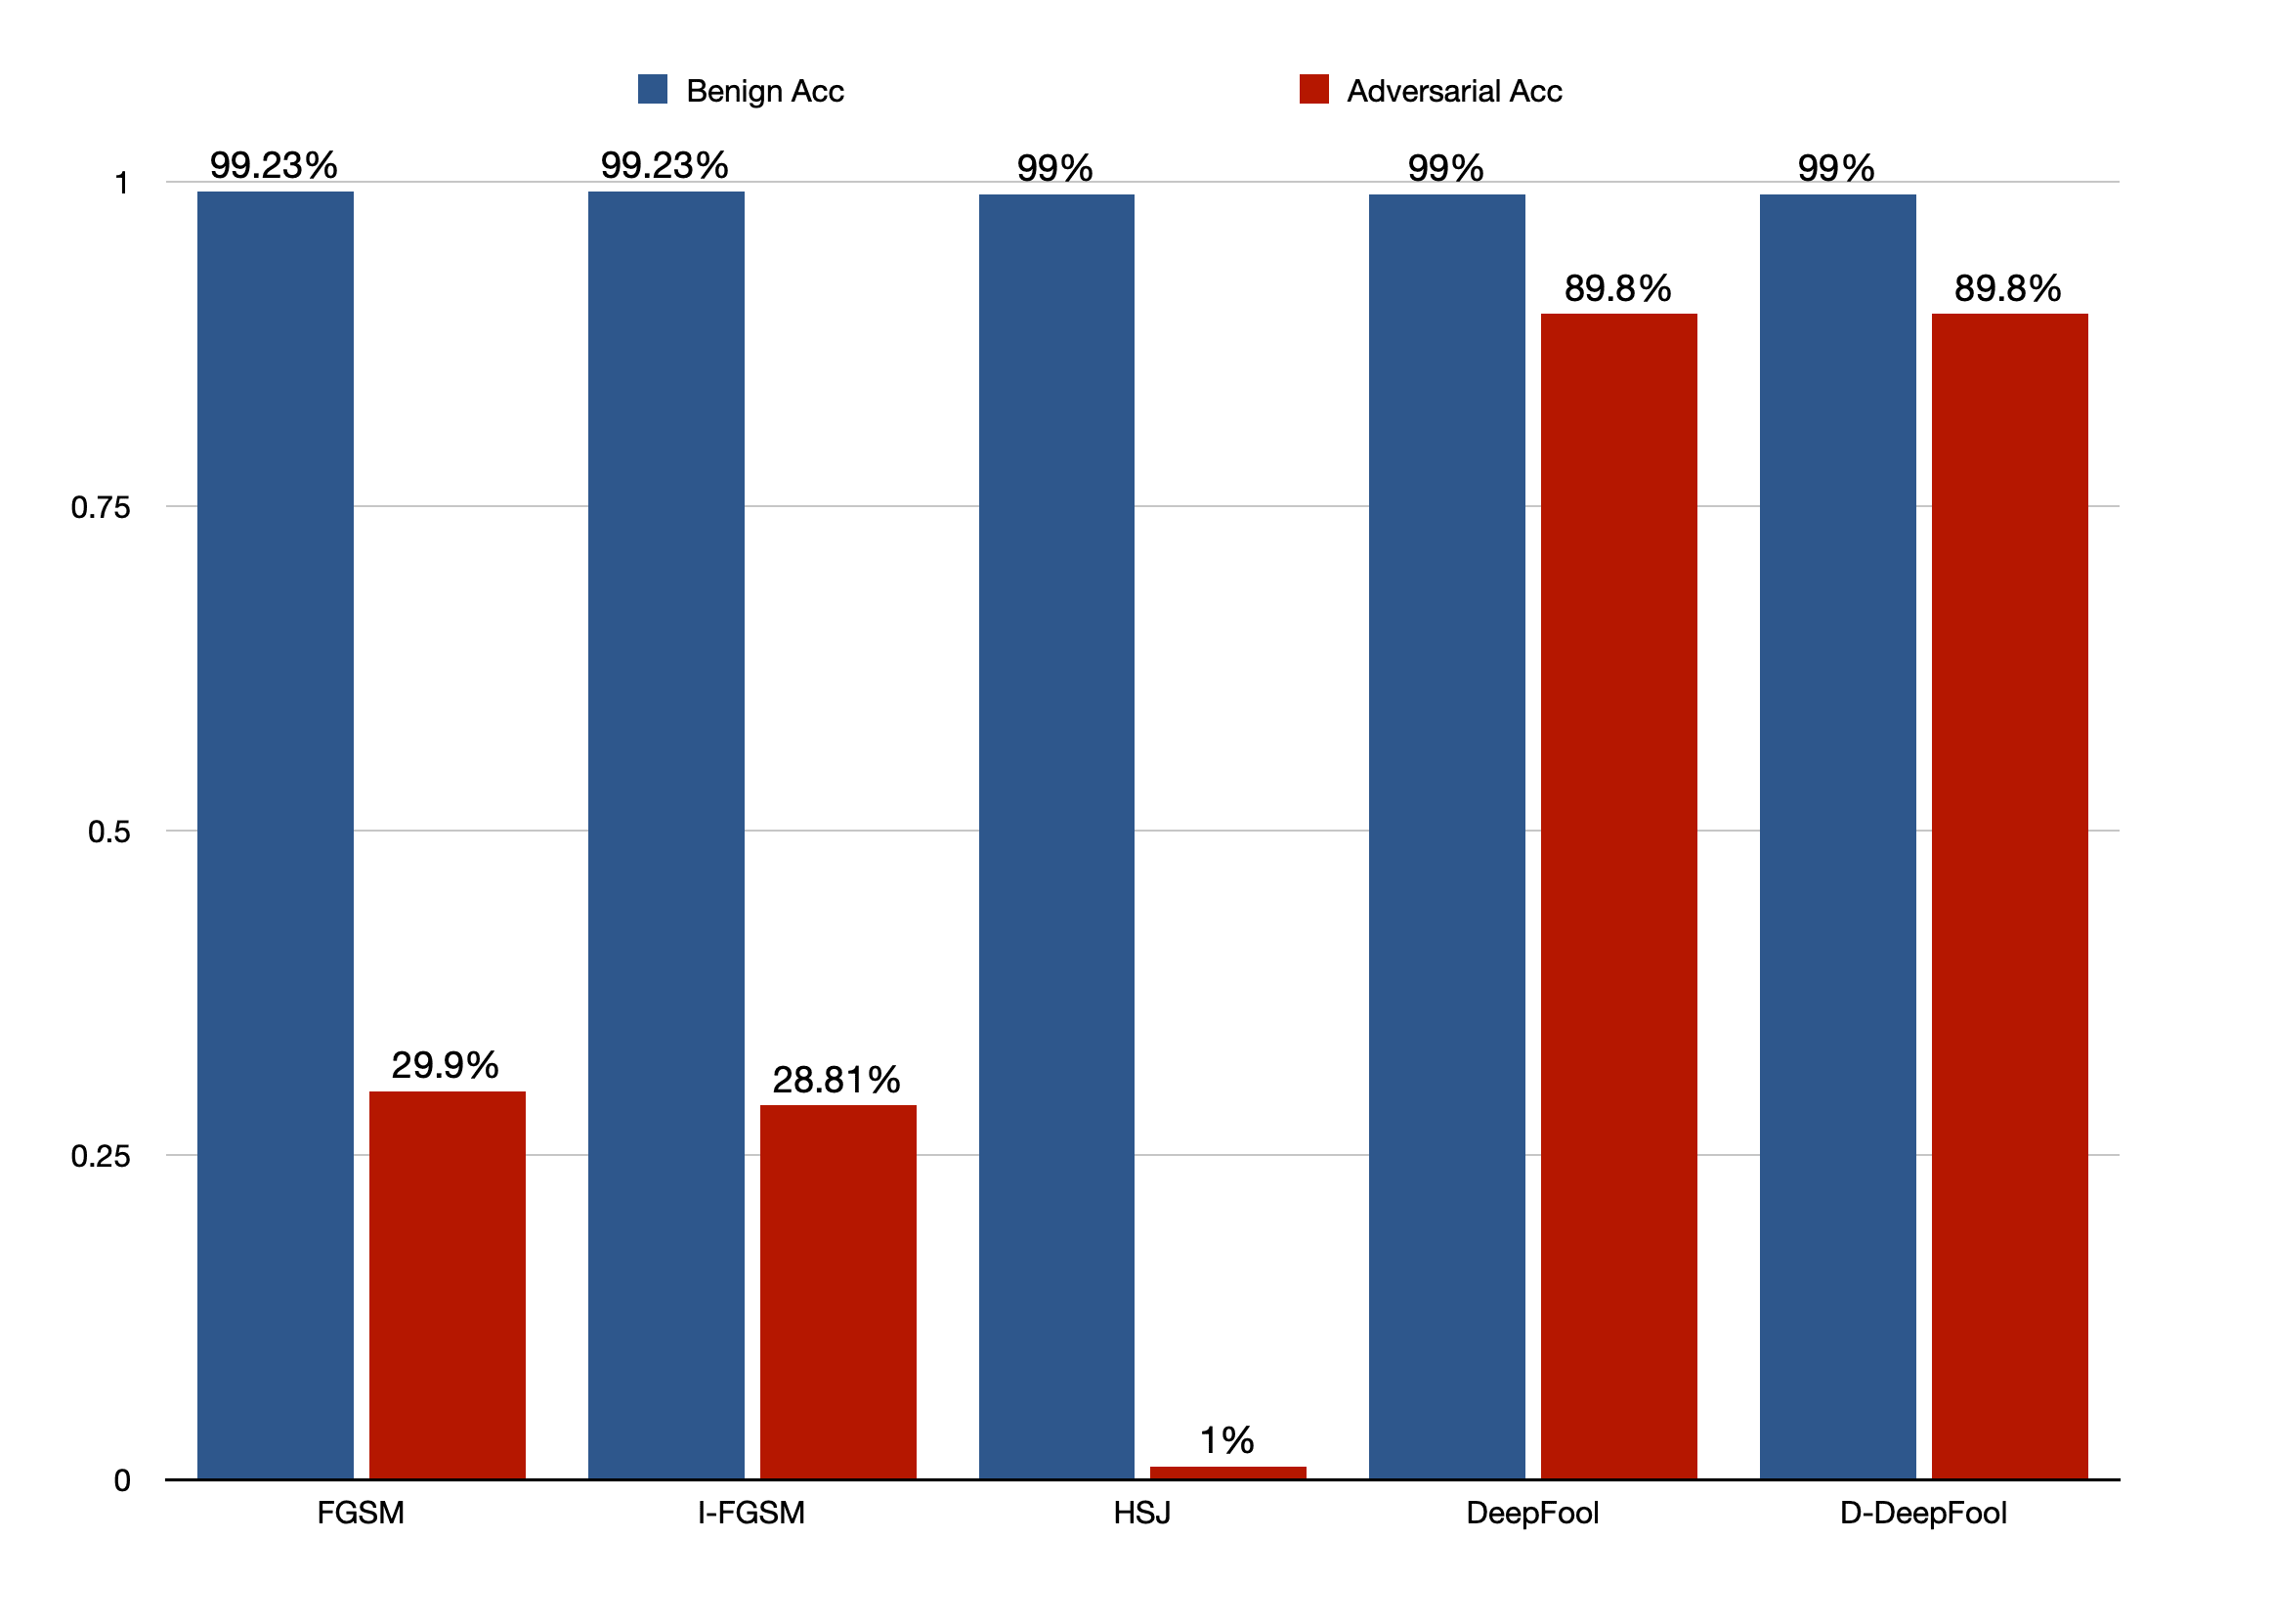
\includegraphics[width = 0.8\textwidth]{{fig/attack_minist_acc.png}}
    \caption{Accuracy comparsion of evasion attack algorithms on \textit{MINIST}}
    \label{attack_minist_acc}
\end{figure}

By observating  [\figurename{\ \ref{attack_minist_acc}}] it can be clearly tell that the presented algorithms are in three different ``levels.'' With \ilc{HSJ} showing the best performance and \ilc{DeepFool} and \ilc{D-DeepFool} showing identical performance, the only interesting question left is if \ilc{FGSM} is significantly different from \ilc{I-FGSM}.

We then try to find the $95 \%$ CI of $E_{\ilc{FGSM}} - E_{\ilc{I-FGSM}}$ with a null hypothesis of they have no difference. Note the sample size of tested \textit{MINIST} is $10000$.

\begin{align*}
    F &= 0.299 - 0.2881 \\
    &= 0.0109 \\
    V(F) &= 0.299(1-0.299)/10000 + 0.2881(1-0.2881)/10000 \\
    &= 0.000041469739\\
    \Rightarrow \sigma &= 0.006439700226 \\
    95 \% \text{CI} &= 0.0109 \pm 1.96 \cdot 0.006439700226 = (-0.001721812443, 0.02352181244)
\end{align*}

With $0$ lies in the $95 \%$ CI, we can't reject the null hypothesis and \ilc{FGSM} and \ilc{I-FGSM} are not different in terms of accuracy performance in this experiment. This is consistent to our understanding of the algorithms as \ilc{I-FGSM} is suppose to be the iterative version of \ilc{FGSM}, it performed slightly ``better'' in number on \textit{adversarial acc} probably just because the adversarial image is generated closer to the decision boundaries of the model and therefore a bit more ``confusing'' -- we will analysize this issue closer with the following budget graph [\figurename{\ \ref{attack_minist_budget}}].

\begin{figure}[H]
    \centering
    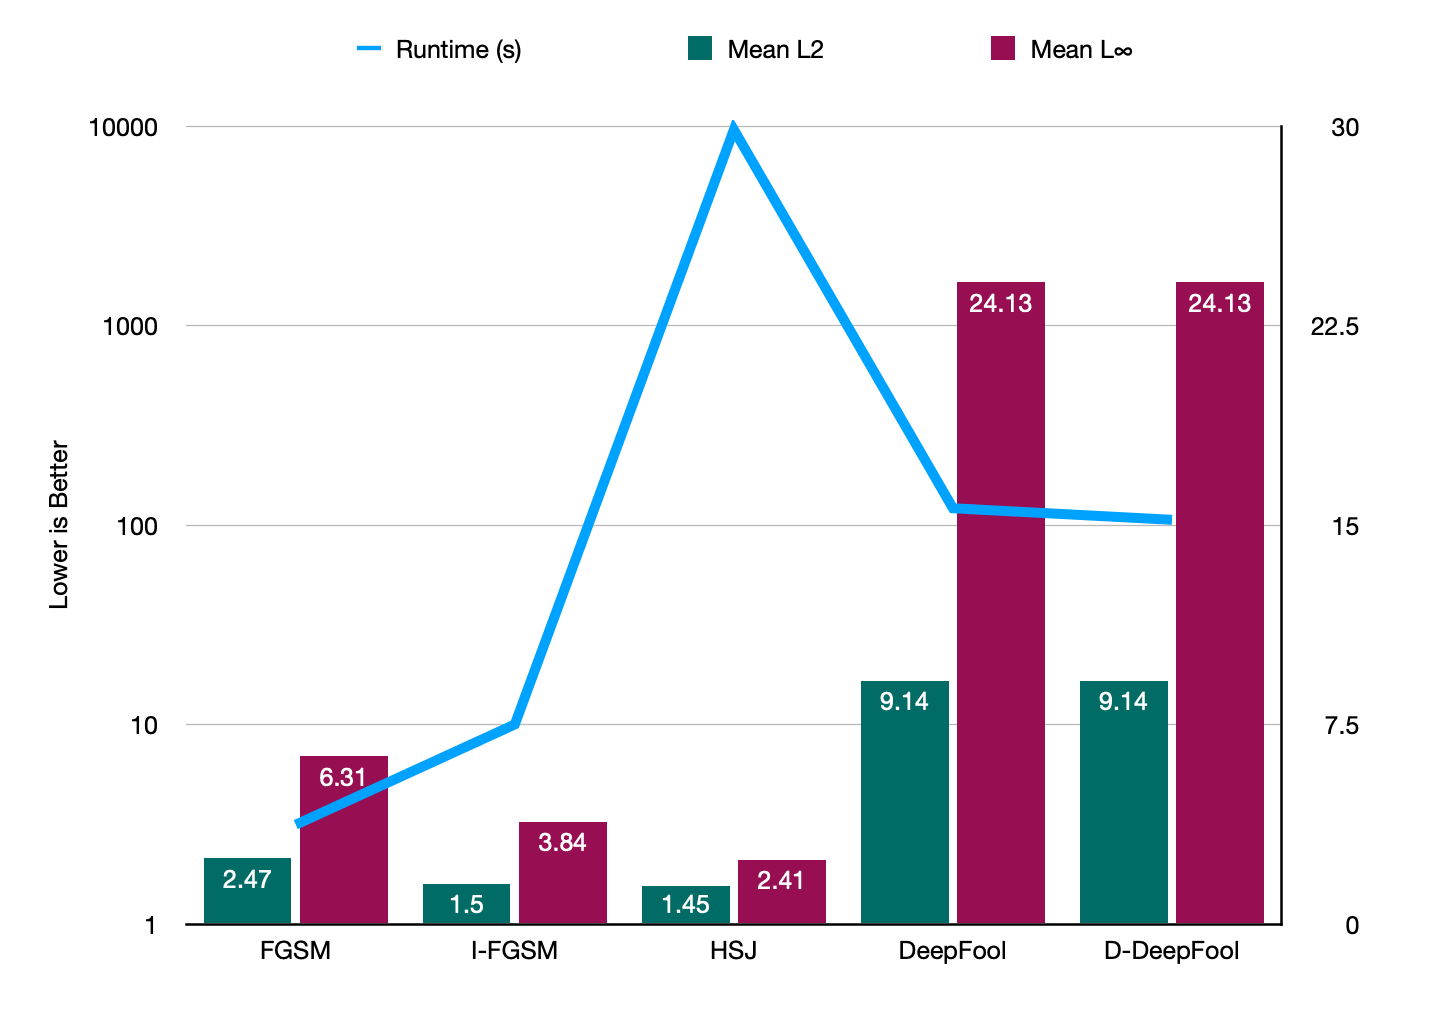
\includegraphics[width = 0.8\textwidth]{{fig/attack_minist_budget.png}}
    \caption{Budget comparsion of evasion attack algorithms on \textit{MINIST}}
    \label{attack_minist_budget}
\end{figure}

By investigating the [\figurename{\ \ref{attack_minist_budget}}] we may confirm our thinking that \ilc{I-FGSM} generated adversarial examples are less aggressive (and thus closer to the decision boundaries), as it has a lower mean $L_2$ and mean $L_\infty$ (we can't do $95 \%$ CI on this as the sample size has no bearing to the perturbation budget).\newline

In our pervious observation on [\figurename{\ \ref{attack_minist_acc}}] we said \ilc{HSJ} has the best performance in terms \textit{adversarial acc}. Now we know that \ilc{HSJ} did such with minimum perturbation budget spent (by having the lowrest mean $L_2$ and mean $L_\infty$ across the board). However, the cost of doing this is very high, the runtime of \ilc{HSJ} is close $100$ times of other algorithm. These observations are also consistent to our understanding of \ilc{HSJ}, as it is doing \textit{binary search} until it crosses the decision boundary -- so it can perserve a high amount semantic from the original image, at the cost of spending a lot of time to find such image.\newline

David please explain a bit on DeepFool as why it perturbed a huge amount while performed not so well, and maybe also why its $L_\infty$ is a lot higher than $L_2$.

\begin{figure}[H]
    \centering
    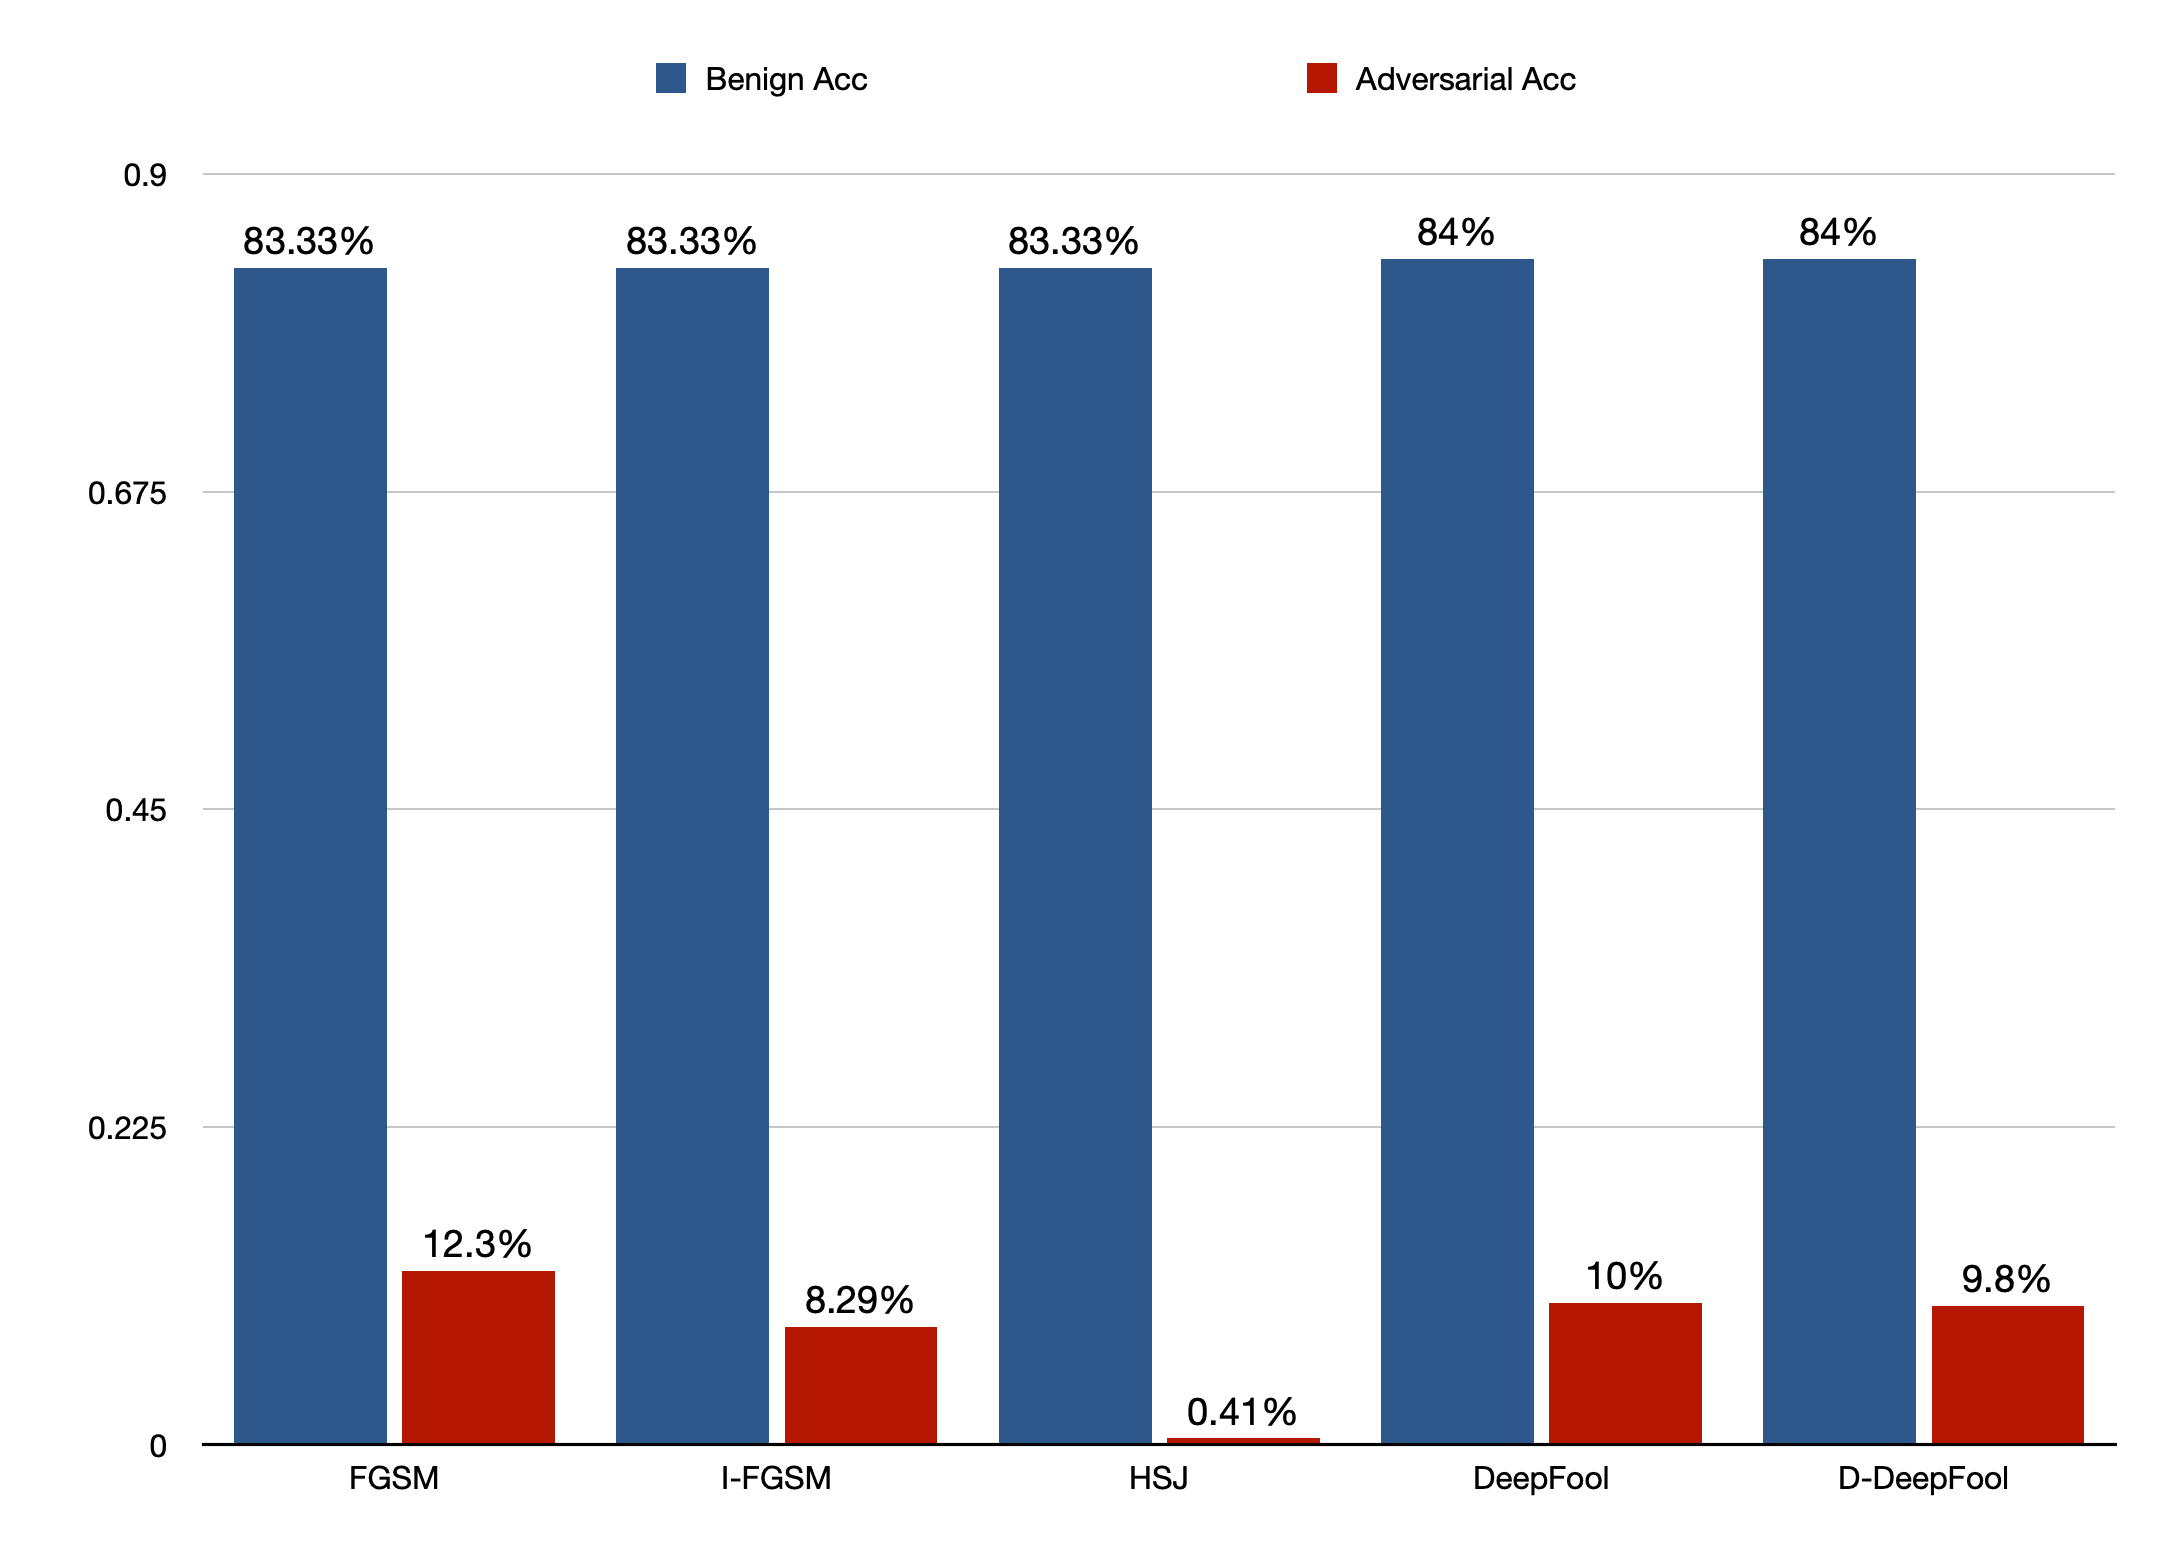
\includegraphics[width = 0.8\textwidth]{{fig/attack_cifar10_acc.png}}
    \caption{Accuracy comparsion of evasion attack algorithms on \textit{CIFAR-10}}
    \label{attack_cifar10_acc}
\end{figure}

We then repeated the same experiment on $100000$ \textit{CIFAR-10} examples and got the result of [\figurename{\ \ref{attack_cifar10_acc}}]. This time we have a different outcome between \ilc{DeepFool} and \ilc{D-DeepFool}, so we will analysis $E_{\ilc{FGSM}} - E_{\ilc{I-FGSM}}$, $E_{\ilc{DeepFool}} - E_{\ilc{D-DeepFool}}$, and $E_{\ilc{I-FGSM}} - E_{\ilc{HSJ}}$ (as they are closer this time). With an aid of a script and a null hypothesis of having no difference, we have:

\begin{itemize}
    \item  $95 \%$ CI of $E_{\ilc{FGSM}} - E_{\ilc{I-FGSM}}$: \ilc{(0.031694853818380074, 0.04850514618161992)}, rejected.
    \item  $95 \%$ CI of $E_{\ilc{DeepFool}} - E_{\ilc{D-DeepFool}}$: \ilc{(-0.006278442326911505, 0.010278442326911509)}, cannot rejected.
    \item  $95 \%$ CI of $E_{\ilc{I-FGSM}} - E_{\ilc{HSJ}}$: \ilc{(0.07325244583218875, 0.08434755416781124)}, rejected.
\end{itemize}

It is a bit suprisized to see the null hypothesis of $E_{\ilc{FGSM}} - E_{\ilc{I-FGSM}} = 0$ can be rejected. This is probably because \textit{CIFAR-10} has more label catagories where \textit{MINIST} only has 10 digits, thus decision boundaries between (more) different labels to be closer. The observation of having an overall lower \textit{benign acc} also confirms this assumption. We will look into it again in the following budget analysis [\figurename{\ \ref{attack_cifar10_budget}}].

Also, with $E_{\ilc{I-FGSM}} - E_{\ilc{HSJ}} = 0$ rejected, we may say that \ilc{HSJ} indeed performs better than \ilc{I-FGSM}.

\begin{figure}[H]
    \centering
    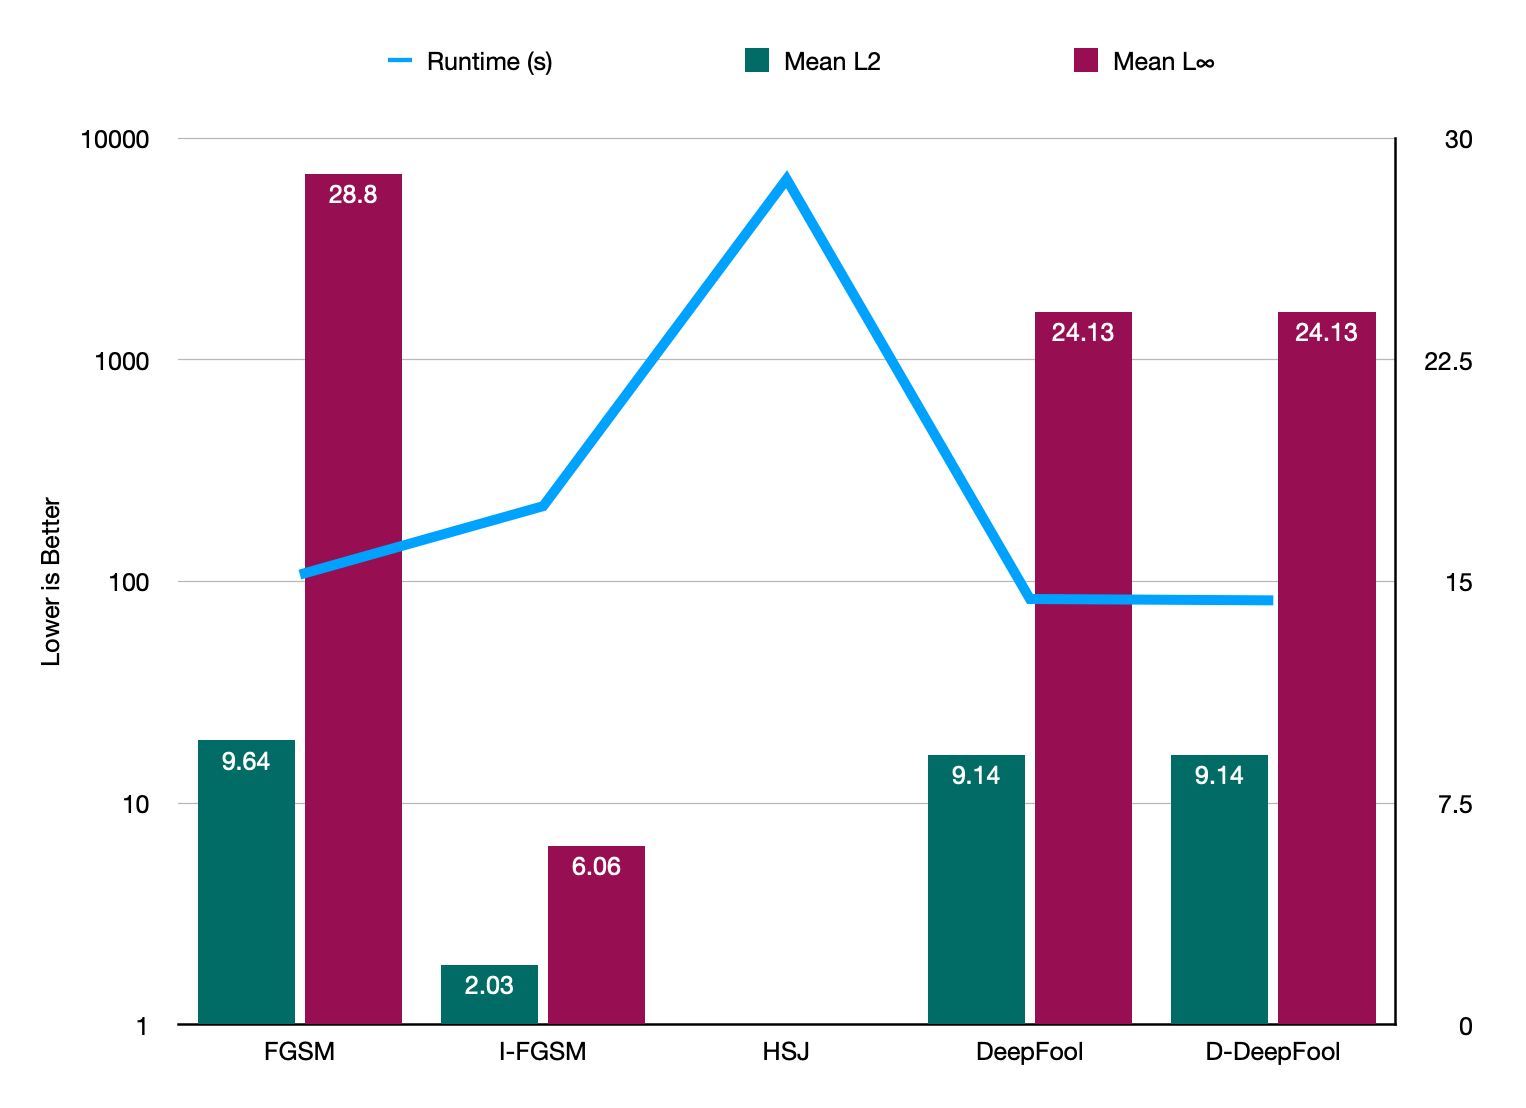
\includegraphics[width = 0.8\textwidth]{{fig/attack_cifar10_budget.png}}
    \caption{Budget comparsion of evasion attack algorithms on \textit{CIFAR-10}}
    \label{attack_cifar10_budget}
\end{figure}

The budget analysis [\figurename{\ \ref{attack_cifar10_budget}}] comfirms our thinking as the perturbation budgets are larger acrossed the board in comparision to \textit{MINIST}. Also all other observation made from the \textit{MINIST} budget graph [\figurename{\ \ref{attack_minist_budget}}] are also true in this \textit{CIFAR-10} budget graph.

\subsubsection{Poisoning}
Please refer to Section \ref{defense_transformer} as we have only one poisoning attack algorithm and want to analysize it in combination with its designated defense: \ilc{Neural Cleanse}.

\subsubsection{Conclusion}

We have made the obersvation of \ilc{HSJ} is having the best \textit{accuracy} performance. With \ilc{HSJ} and \ilc{I-FGSM} being more successful on controlling their perturbation budget -- due to their iterative nature -- and therefore probably are overall more reliable attacks as they can generate more effective (i.e. more confuse to a modal) adversarial examples while preserve better semantic of the original benign image (i.e. the pertubation is less obvious to human's eyes).

Note we also discovered \ilc{I-FGSM} and \ilc{HSJ} are computationally-heavy (especially the latter), due to their iterative nature and the need of many binary search operations in the case of \ilc{HSJ}. So it is suspected this sort of attacks can be better prevented by implementing flow control mechanism of the model \ilc{predict()} API -- as without enough steps of iterations, these two algorithms won't easily find the decision boundary of the model.\newline

\ilc{DeepFool} and \ilc{D-DeepFool} have shown very similar performance across this section of experiments and their performance are considerably lacking both in terms of \textit{adversarial acc} and \textit{perturbation budget}. David, please again summarize a bit here.

\subsection{Defense Algorithms}

The setup of algorithms and environment remain consistent to Section \ref{attack_algo}, with the exception of we ran \ilc{HSJ} with the params of \ilc{max\_iter=8, max\_eval=100, init\_eval=10} due to resource concern.\newline


\noindent Unless specifically addressed, the base line model is a the pretrained model of dataset wrapped in \ilc{ART}'s \ilc{KerasClassifier}; and the testing sample size of datasets are $500$ (per each databset).

\subsubsection{Detector}

\begin{figure}[H]
    \centering
    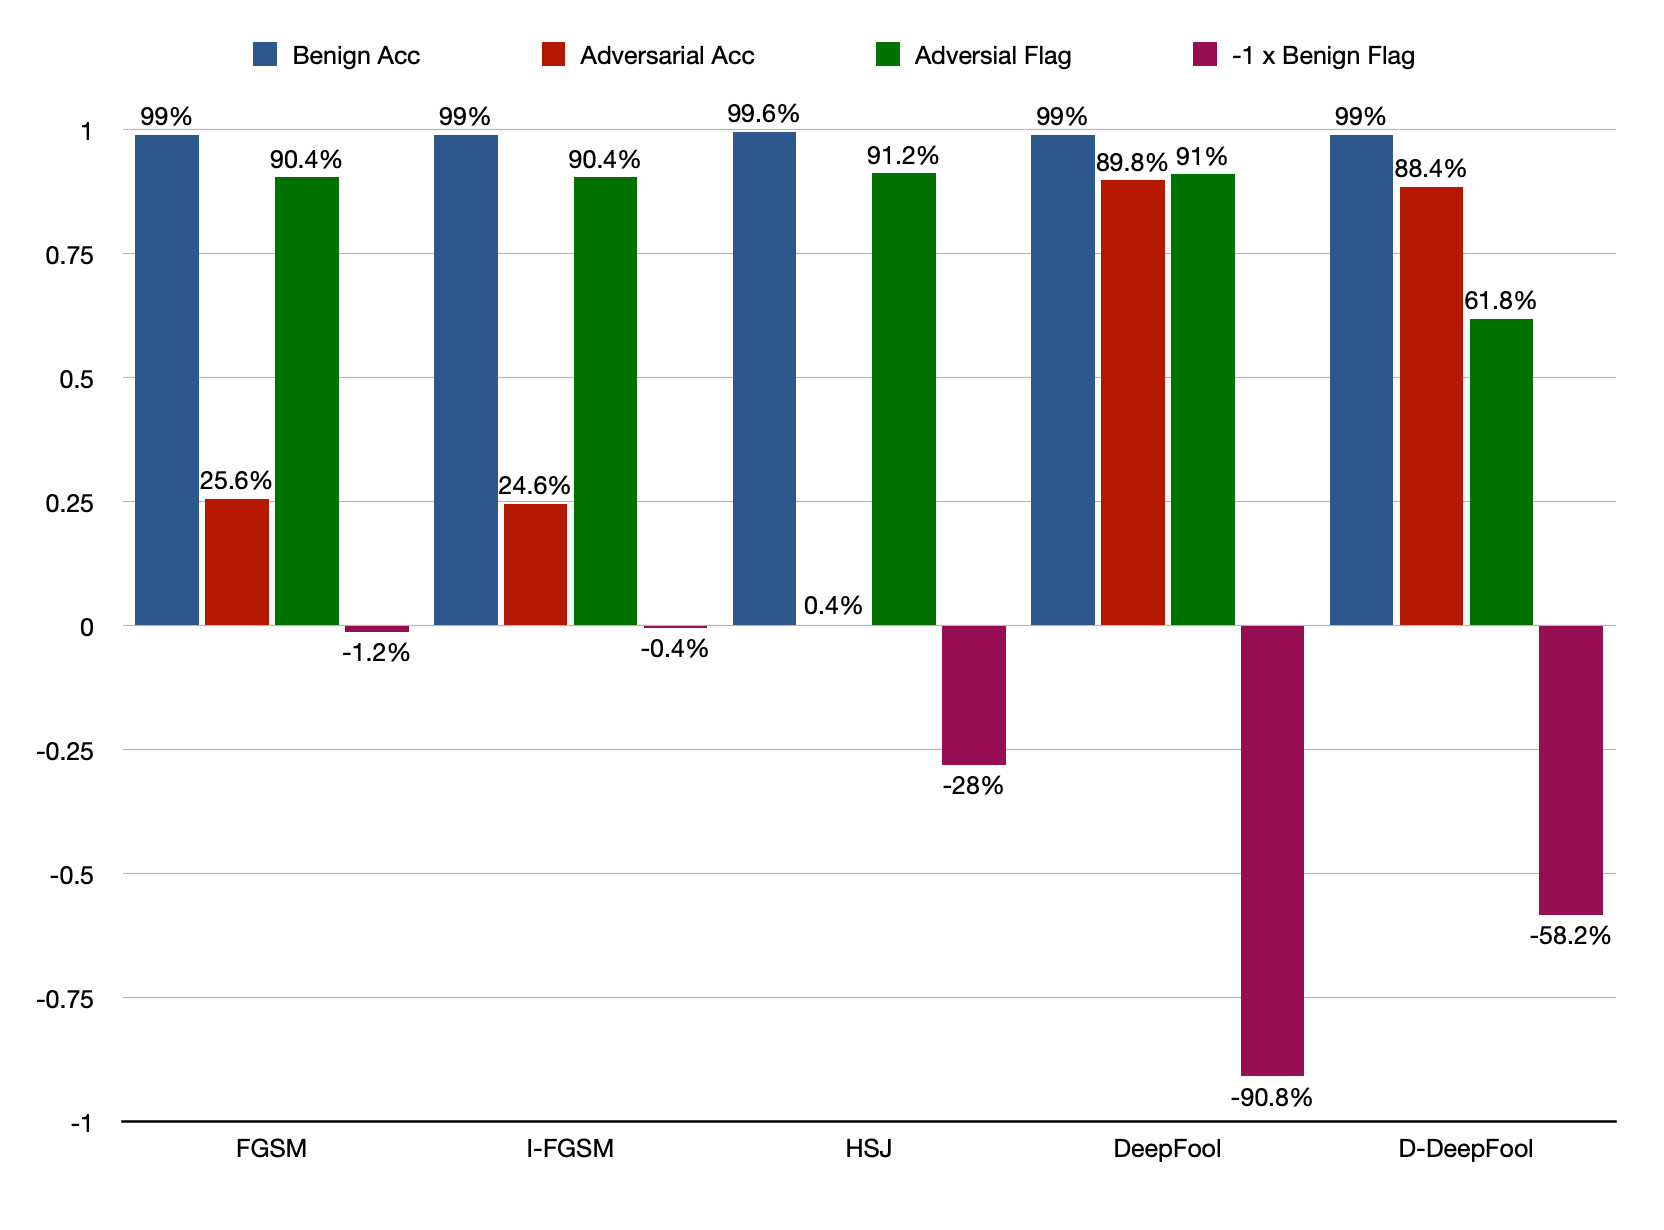
\includegraphics[width = 0.8\textwidth]{{fig/bd_minist_acc.png}}
    \caption{Effectiveness comparision of evasion attack algorithms v. \ilc{Binary Input Detector} on \textit{MINIST}}
    \label{bd_minist_acc}
\end{figure}

\ilc{Binary Input Detector} a.k.a \ilc{BID} is algorithm that detects and flags adversarial examples out of a dataset. Since the workflow of our experiment is to get the \textit{benign acc} with original benign examples, then make them into adversarial exmaples to get the \textit{adversarial acc}, then we ask \ilc{BID} to run on both the benign example set and the adversarial example set.

In the adversarial example set, \ilc{BID} should aim for a $100 \%$ as every input example of the set is adversarial; vice versa, \ilc{BID} should aim for a $0 \%$ in the benign example set as none of the input exmaple are adversarial -- we times this benign flagging percentage with an $-1$ do show that it is a negative impact.\newline

\noindent First, we may tell there is much difference on \textit{adversarial flag} except for \ilc{D-DeepFool}, as we have $95 \%$ of $E_{\ilc{HSJ}} - E_{\ilc{FGSM}}$ (the biggest difference on \textit{adversarial flag} excluding \ilc{D-DeepFool}) to be \ilc{(-0.027824596689983806, 0.04382459668998382)}, so we cannot reject the null hypothesis of \ilc{FGSM, I-FGSM, HSJ, DeepFool} having no significant difference on \textit{adversarial flag}.\newline

Thus, the interest is left to \textit{benign flag}, we cannot rejected $E_{\ilc{FGSM}} - E_{\ilc{I-FGSM}} = 0$ by having a  $95 \%$ of \ilc{(-0.0030318578671047047, 0.019031857867104707)}. But there are significant differences between \ilc{HSJ, DeepFool, D-DeepFool} on \textit{benign flag} as we have tested the $95 \%$ of $E_{\ilc{HSJ}} - E_{\ilc{FGSM}} = 0$ (second smallested difference on \textit{benign flag}) to be \ilc{(0.22750277615440784, 0.3084972238455922)} on \textit{benign flag}. We think this can be better explained by investigating the [\figurename{\ \ref{bd_minist_budget}}] graph.


\begin{figure}[H]
    \centering
    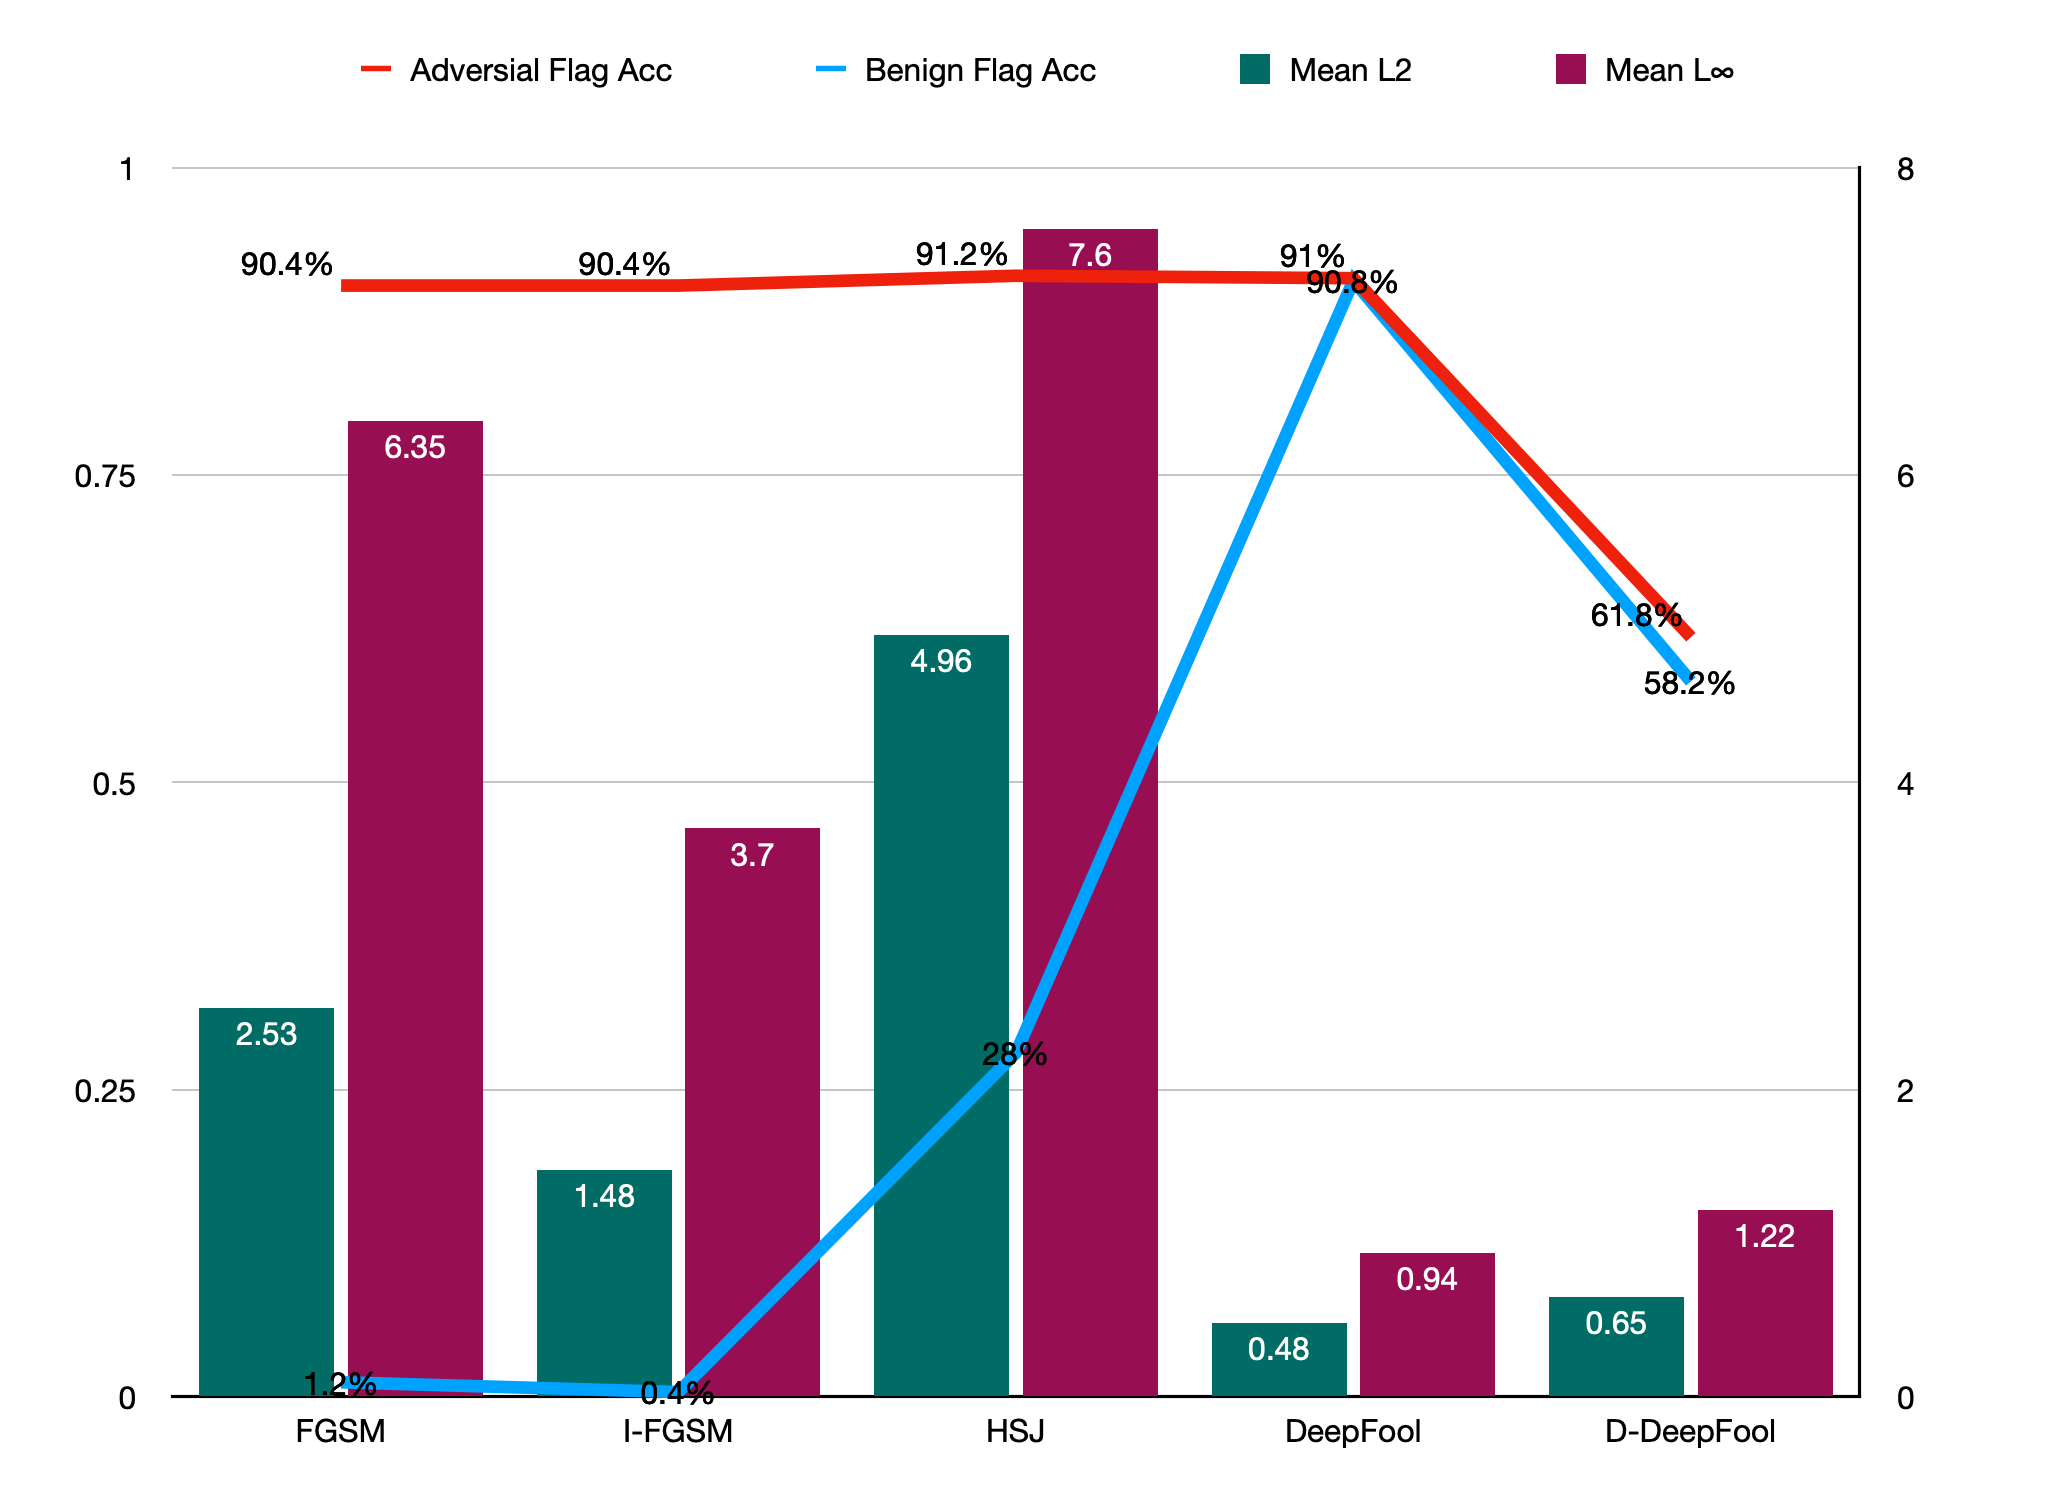
\includegraphics[width = 0.8\textwidth]{{fig/bd_minist_budget.png}}
    \caption{Budget comparision evasion attack algorithms v. \ilc{Binary Input Detector} on \textit{MINIST}}
    \label{bd_minist_budget}
\end{figure}

By investigating the [\figurename{\ \ref{bd_minist_budget}}] graph, it can be tell there is a clearly correlation between the \textit{pertubation budget} and the \textit{adversarial flag} or \textit{benign flag} (e.g., \ilc{D-DeepFool}). This is in fact very intuitive as less \textit{pertubation budget}  means the generated adversarial examples have perserved more semantics or their benign origins, thus making \ilc{BID} hard to distinguish wheather an example is benign or not.

However, it remainds unknow why \ilc{D-DeepFool} has a much lesser \textit{benign flag} and \textit{adversarial flag} in comparision to \ilc{DeepFool}. David please have some input here thanks.


\begin{figure}[H]
\minipage{0.6\textwidth}
    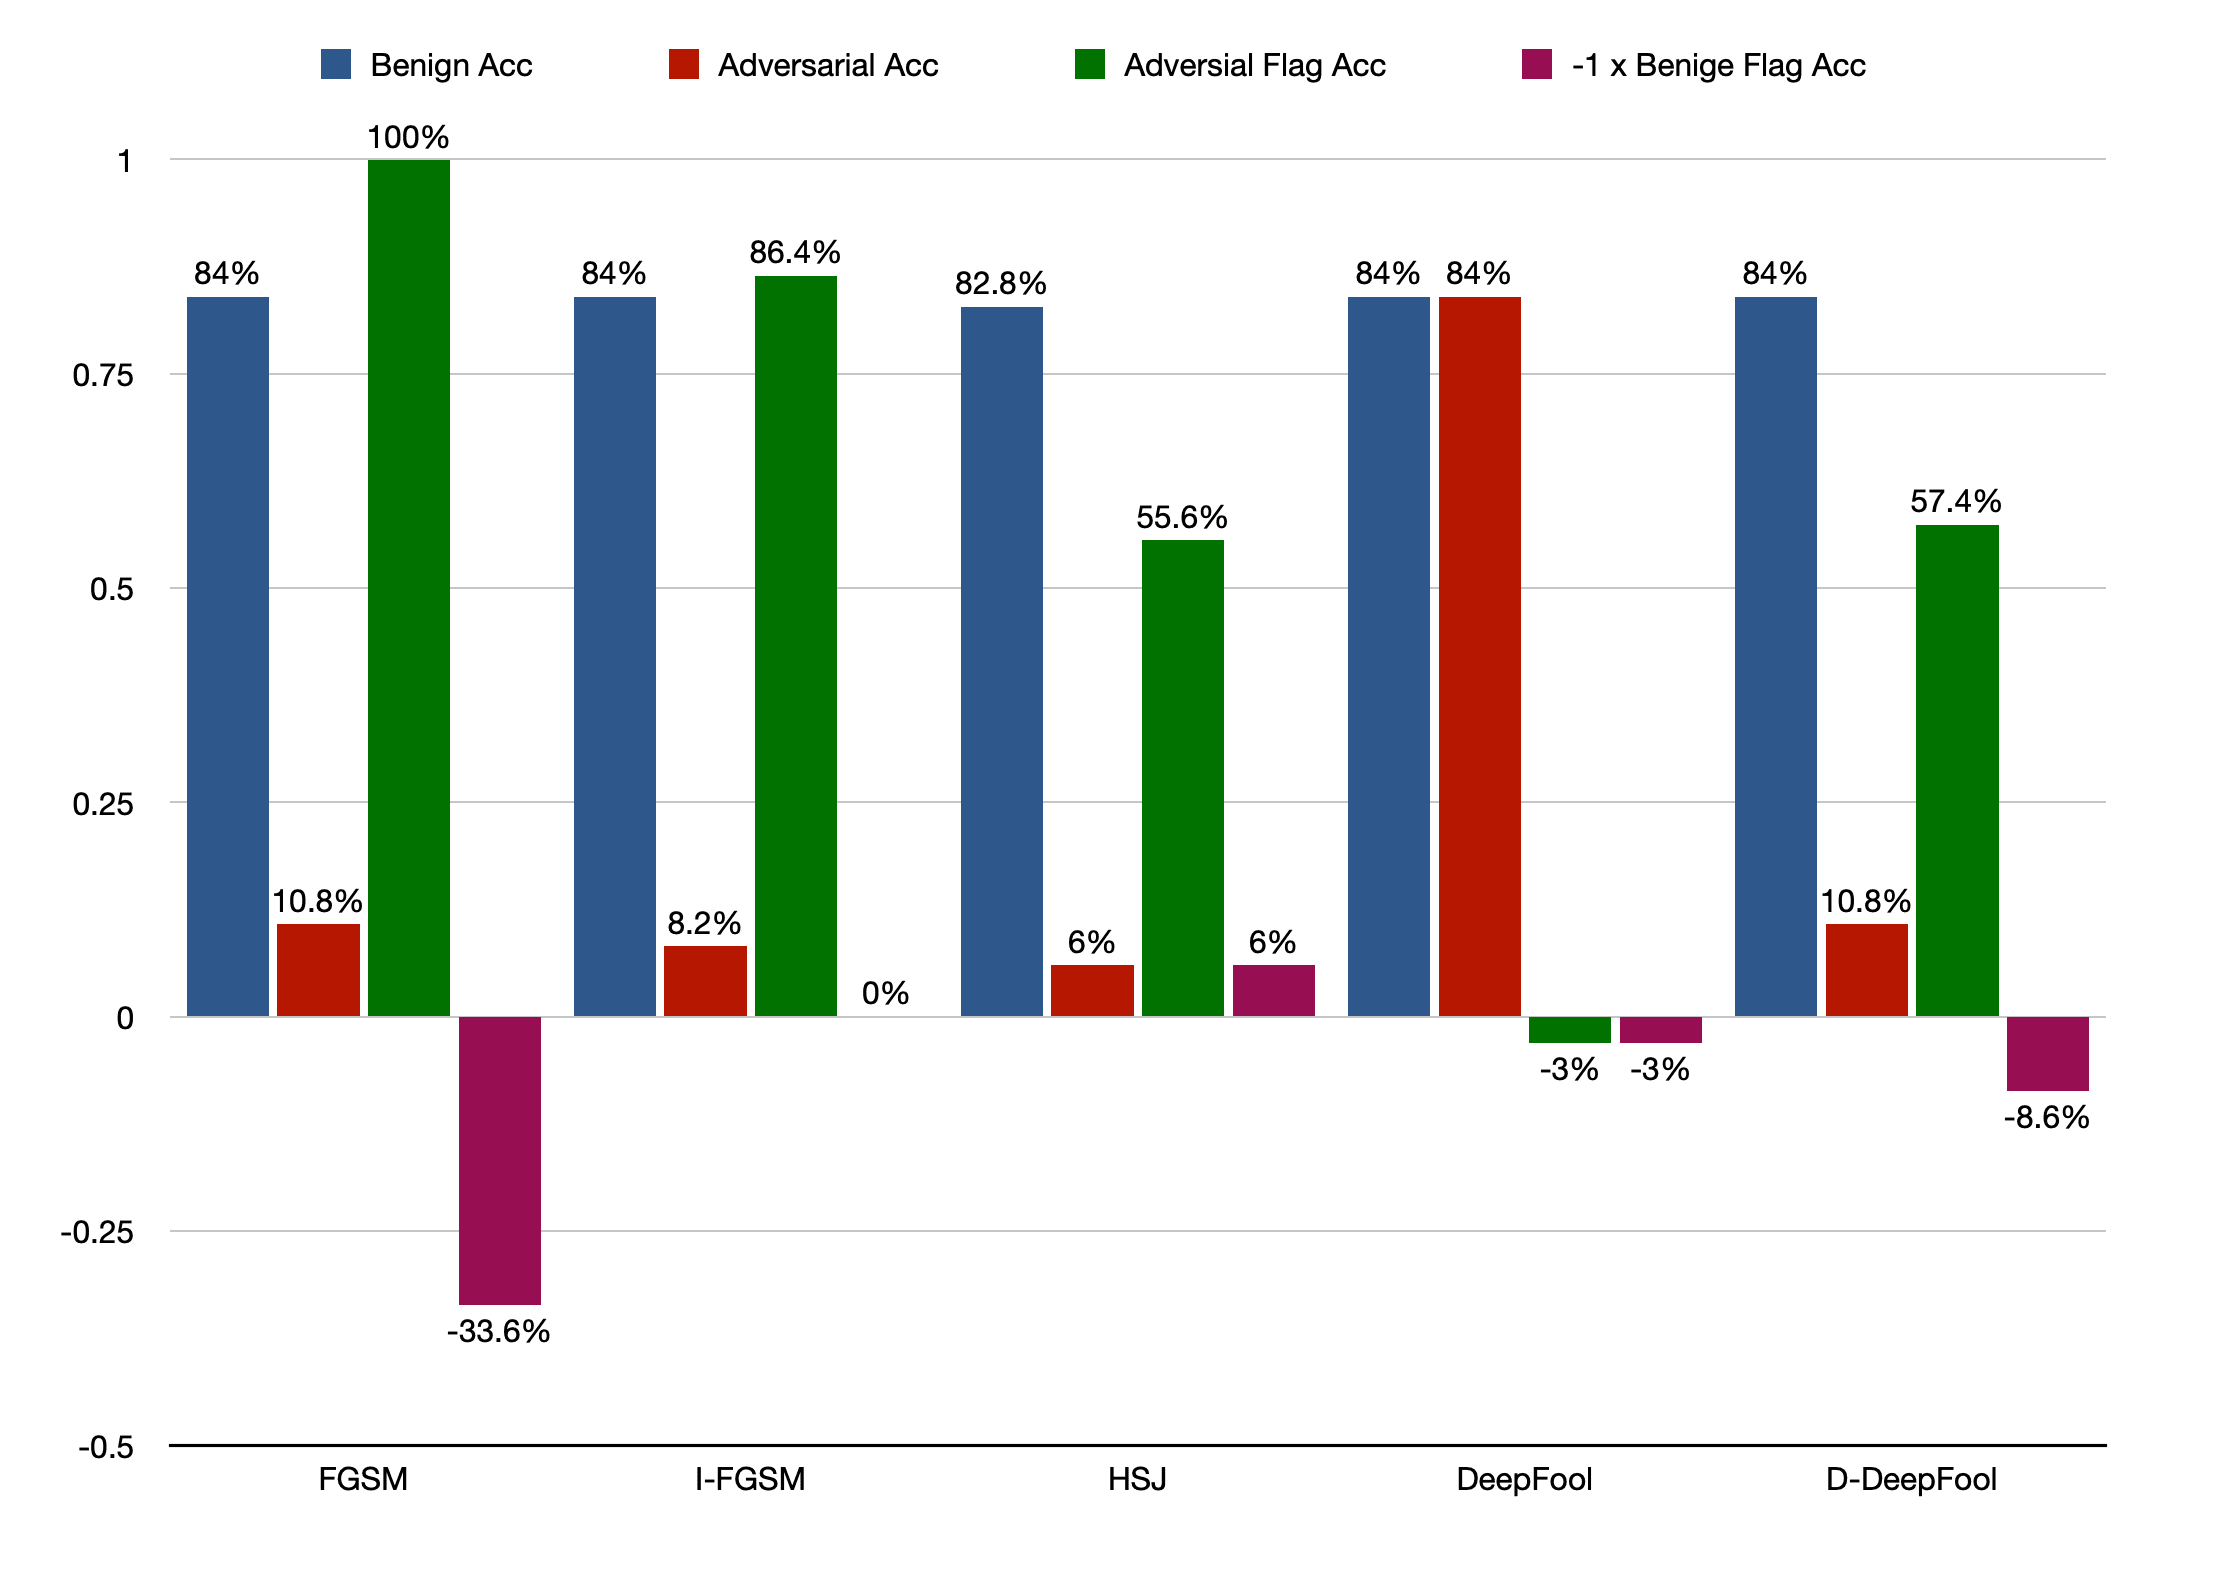
\includegraphics[width=0.8\textwidth]{{fig/bd_cifar10_acc.png}}
    \caption{Effectiveness comparision}
    \label{bd_cifar10_acc}
\endminipage\hfill
\minipage{0.6\textwidth}
    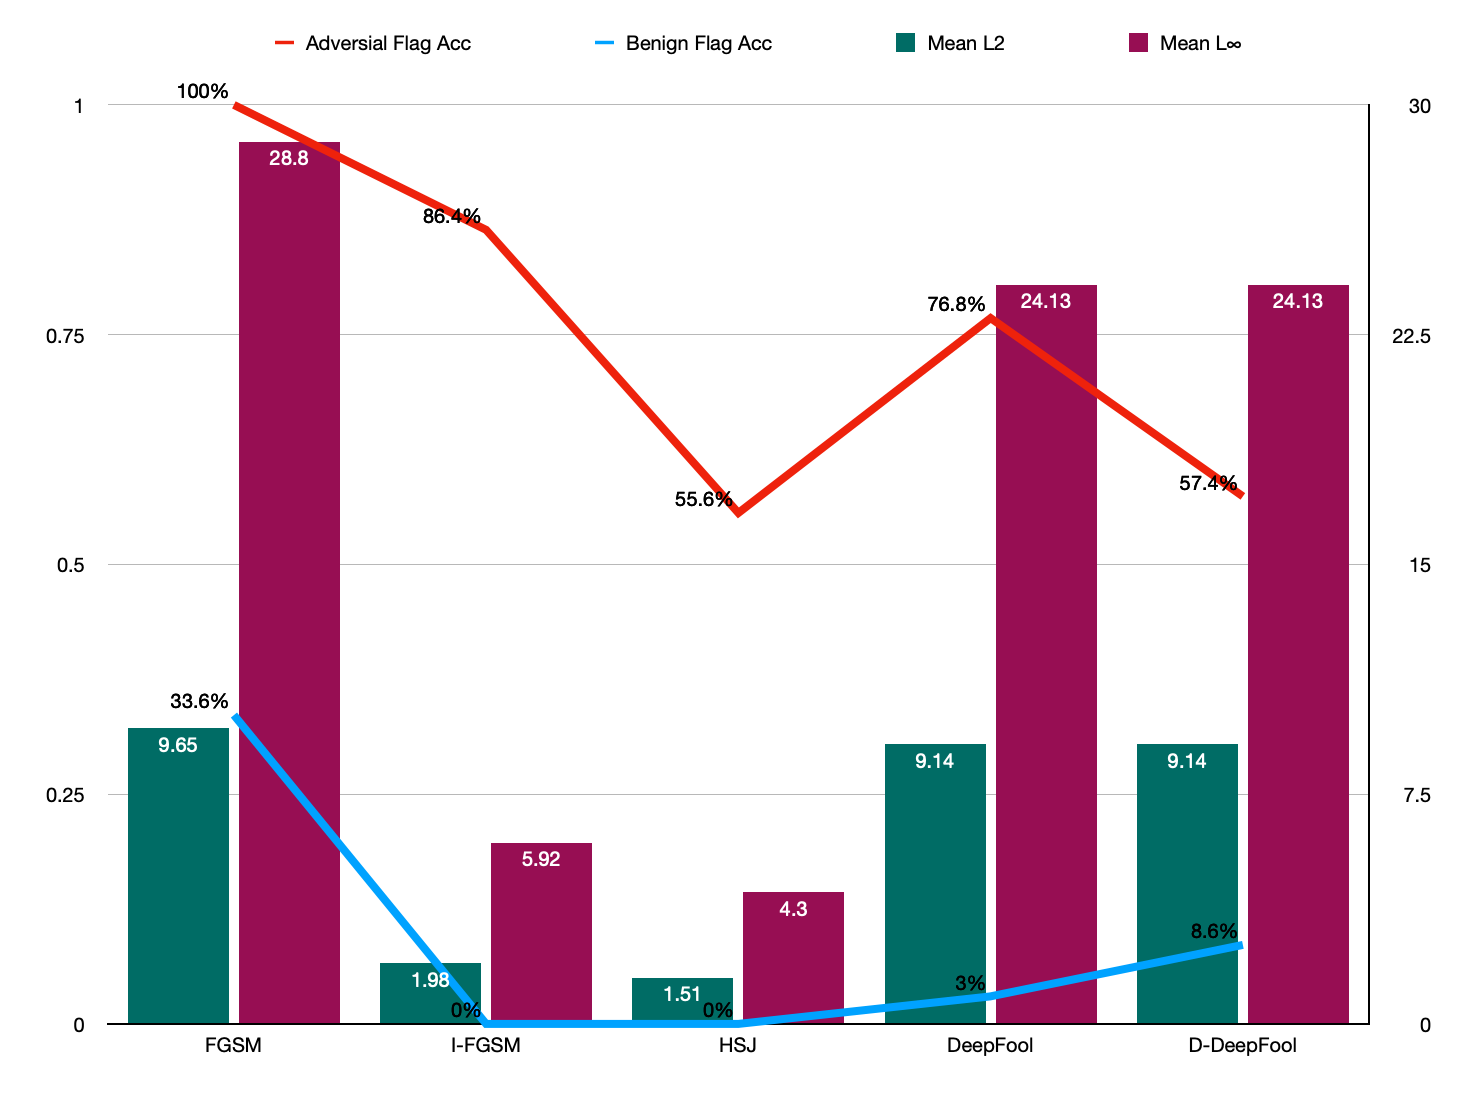
\includegraphics[width=0.8\textwidth]{{fig/bd_cifar10_budget.png}}
    \caption{Budget comparision}
    \label{bd_cifar10_budget}
\endminipage
\caption*{Evasion attack algorithms v. \ilc{Binary Input Detector} on \textit{CIFAR-10}}
\end{figure}


Our discovary continues uphold on the \textit{CIFAR-10} dataset as algorithms with lower \textit{pertubation budget} gets flagged less (regardless adversarial or benign).

However, this time it is \ilc{I-FGSM} and \ilc{HSJ} having the least \textit{pertubation budget}. This is in fact resonable due to their iterative nature. We looked into our experiment and realized it is because \ilc{HSJ} was running on a test set of $250$ examples\footnote{We have to reduce the size as \ilc{BID} needs to generate the adversarial images twices}, in combinations with \ilc{max\_iter = 8}, the algorithm might not have enough iterations and random move to detect the decision boundaries of \textit{MINIST}, which can be a lot harder to detect as they all have pure-color backgrounds.


\subsubsection{Pre-processor}


\begin{figure}[H]

\minipage{0.6\textwidth}
    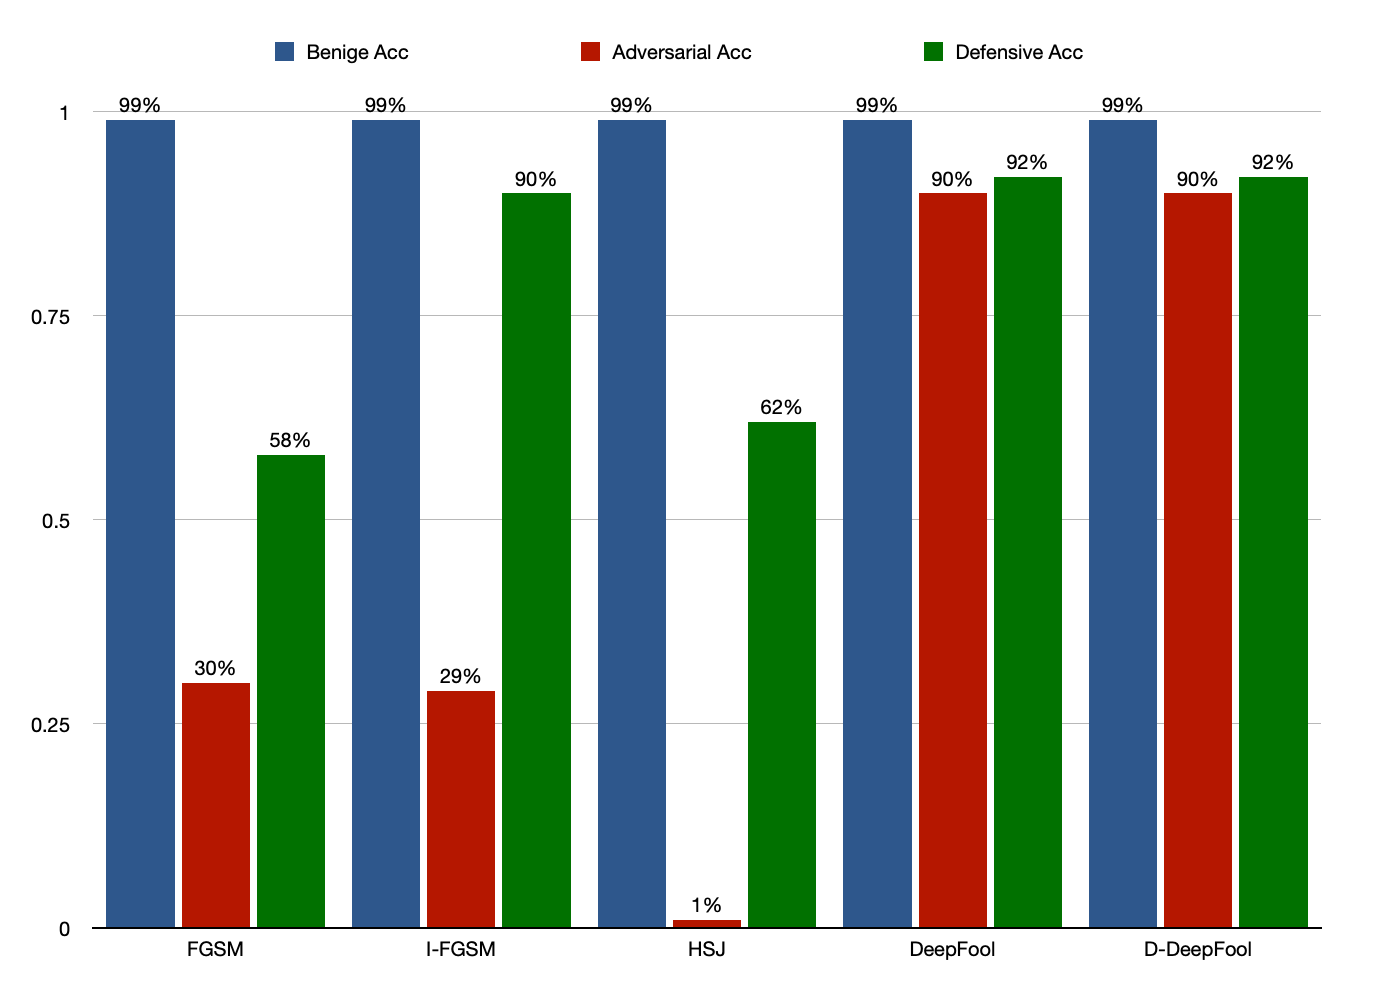
\includegraphics[width = 0.8\textwidth]{{fig/ss_minist_acc.png}}
    \caption{Effectiveness comparision}
    \label{ss_minist_acc}
\endminipage\hfill
\minipage{0.6\textwidth}
    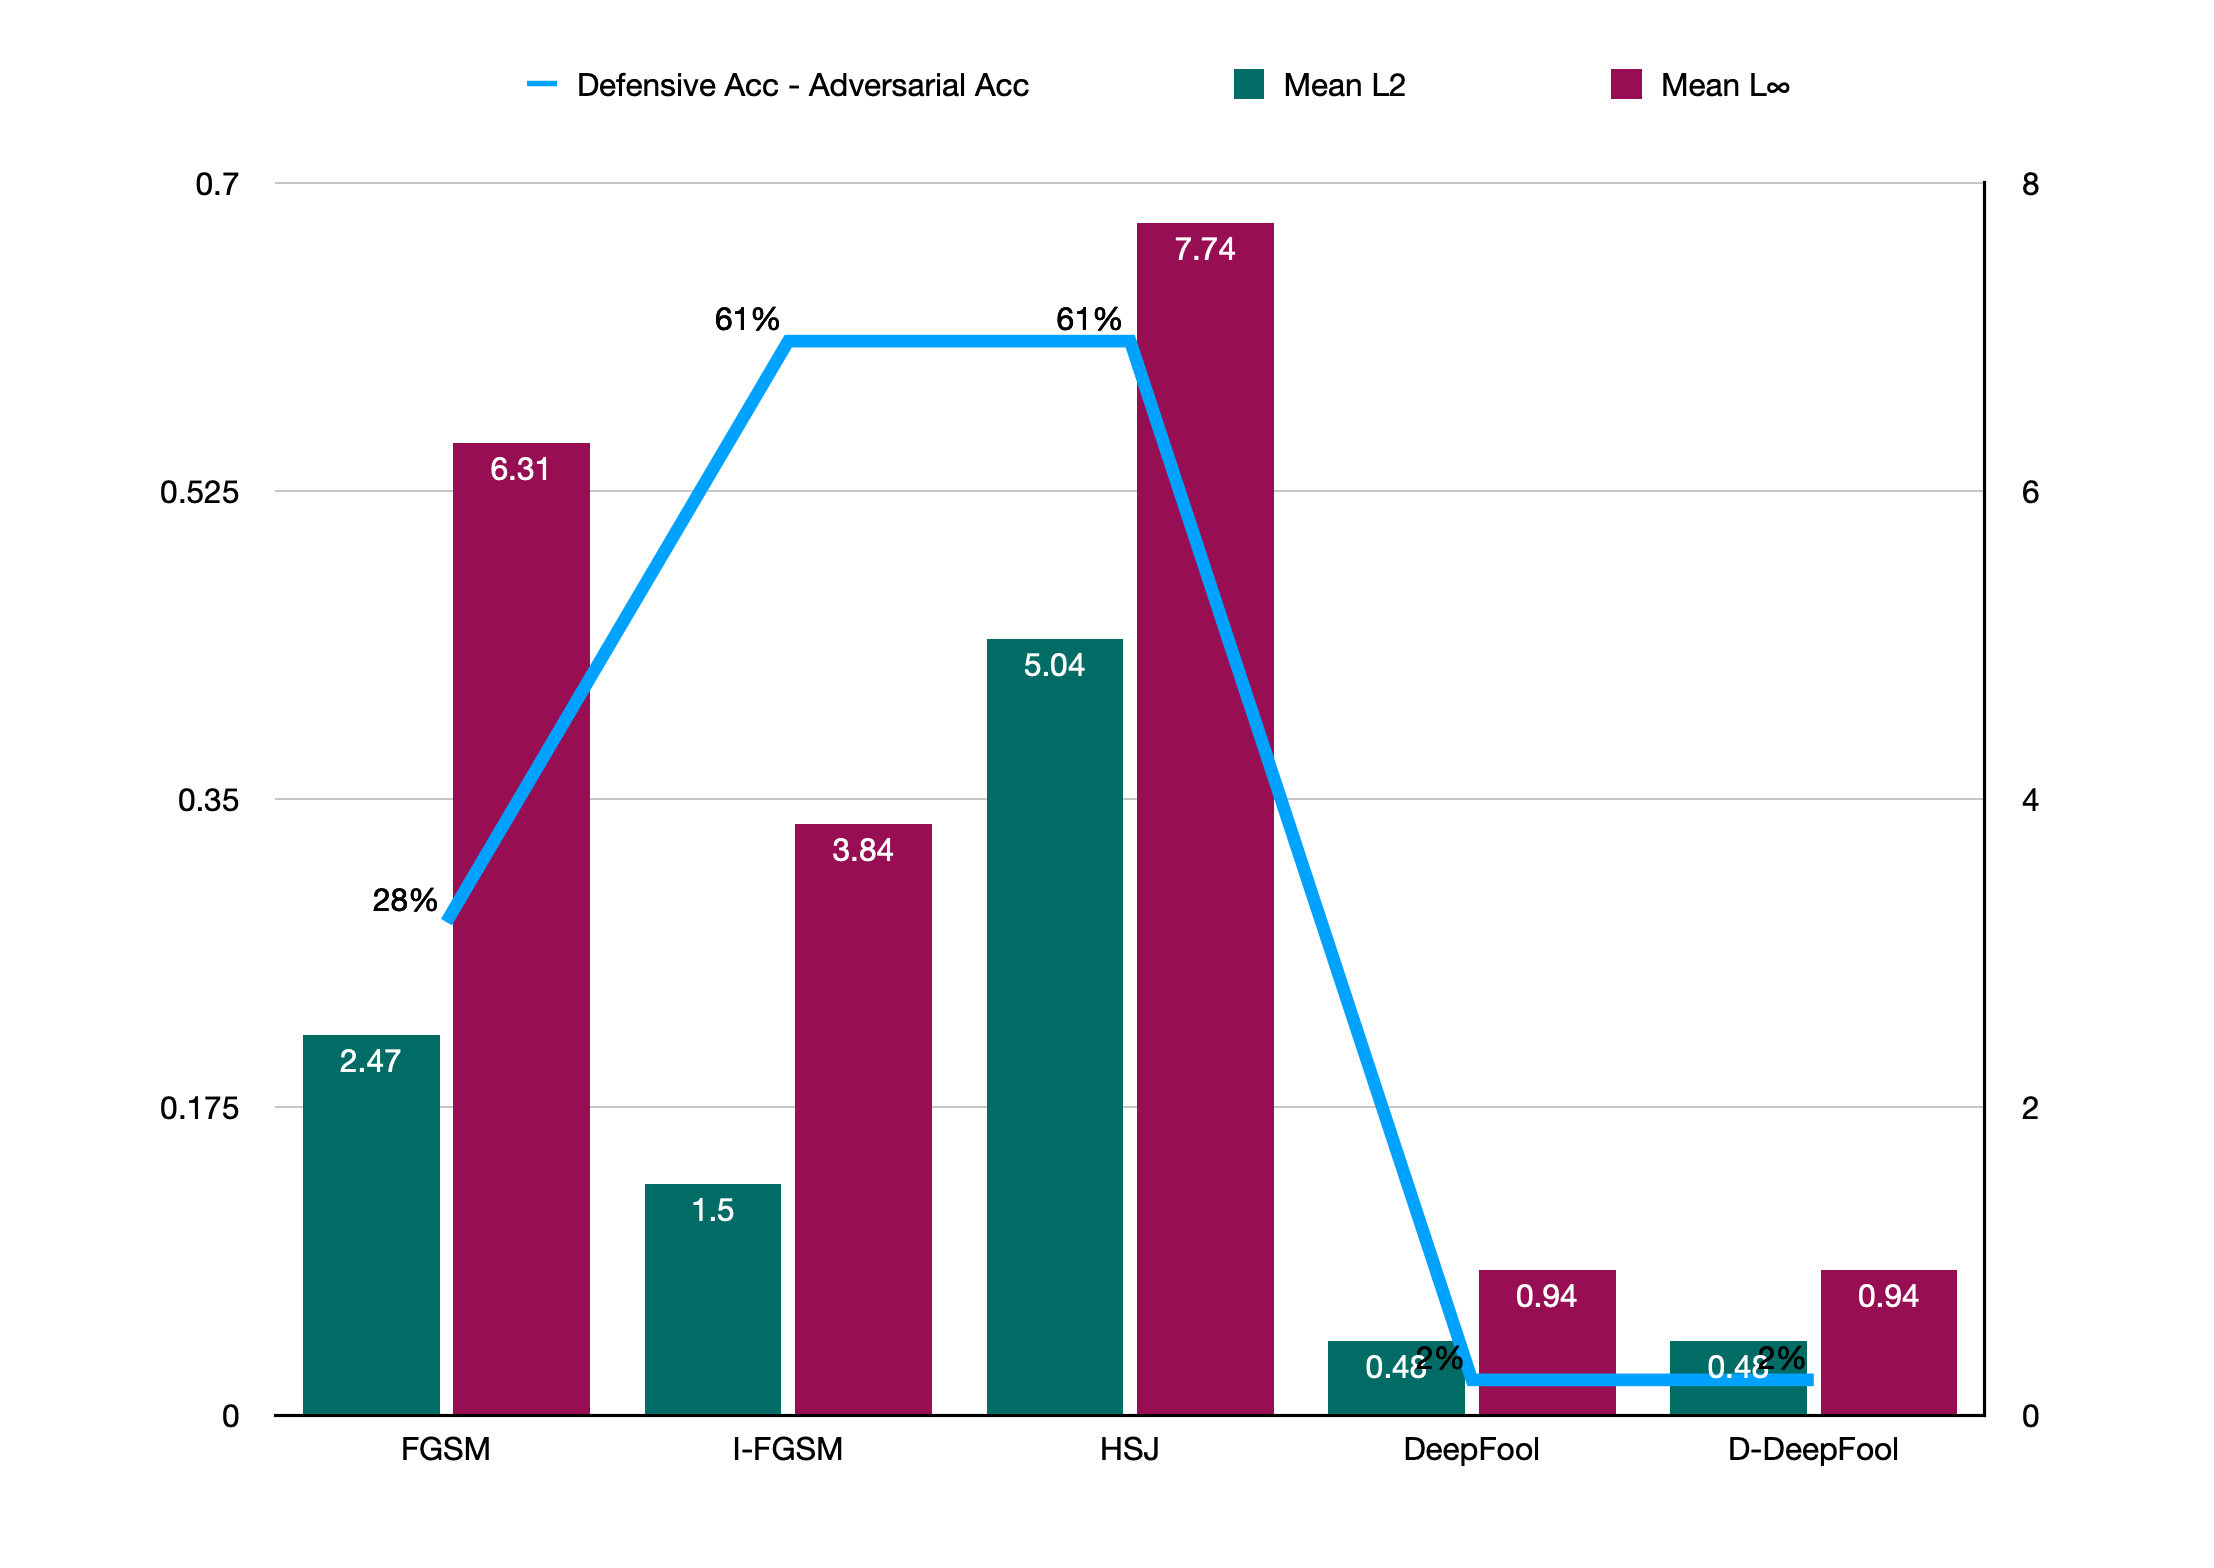
\includegraphics[width = 0.8\textwidth]{{fig/ss_minist_budget.png}}
    \caption{Budget comparision}
    \label{ss_minist_budget}
\endminipage
\caption*{Evasion attack algorithms v. \ilc{Spatial Smoothing} on \textit{MINIST}}
\end{figure}

\begin{figure}[H]

\minipage{0.6\textwidth}
    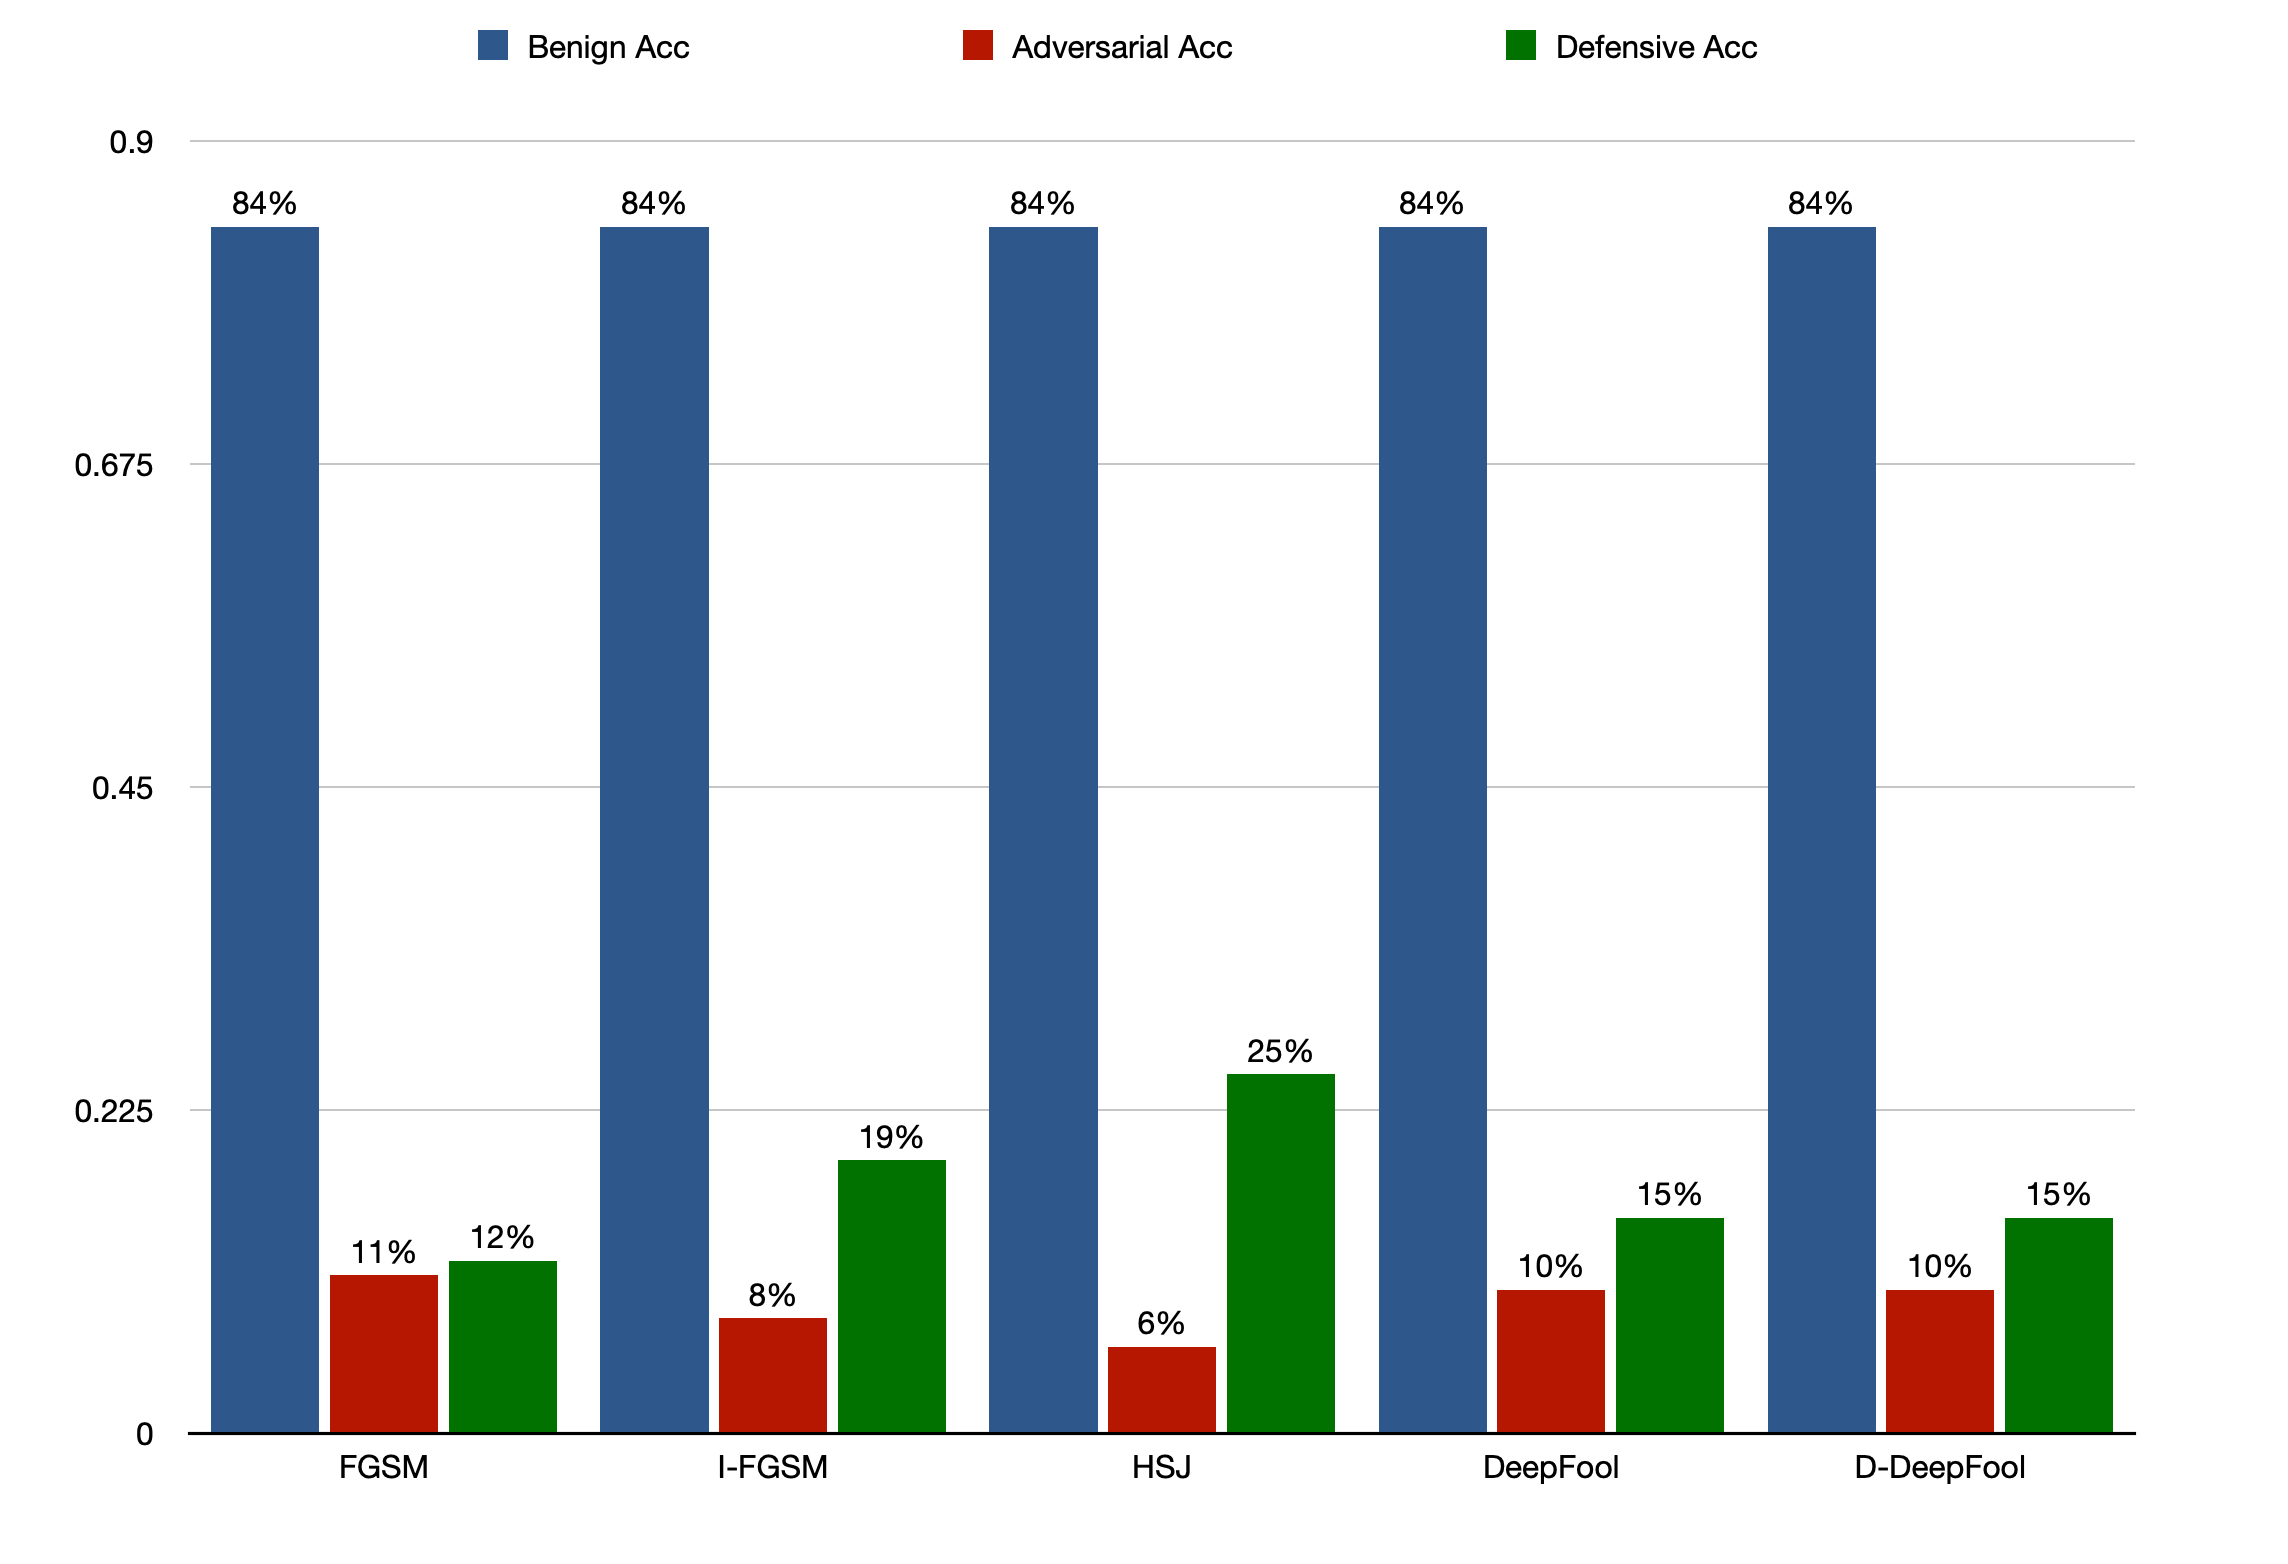
\includegraphics[width = 0.8\textwidth]{{fig/ss_cifar10_acc.png}}
    \caption{Effectiveness comparision}
    \label{ss_cifar10_acc}
\endminipage\hfill
\minipage{0.6\textwidth}
    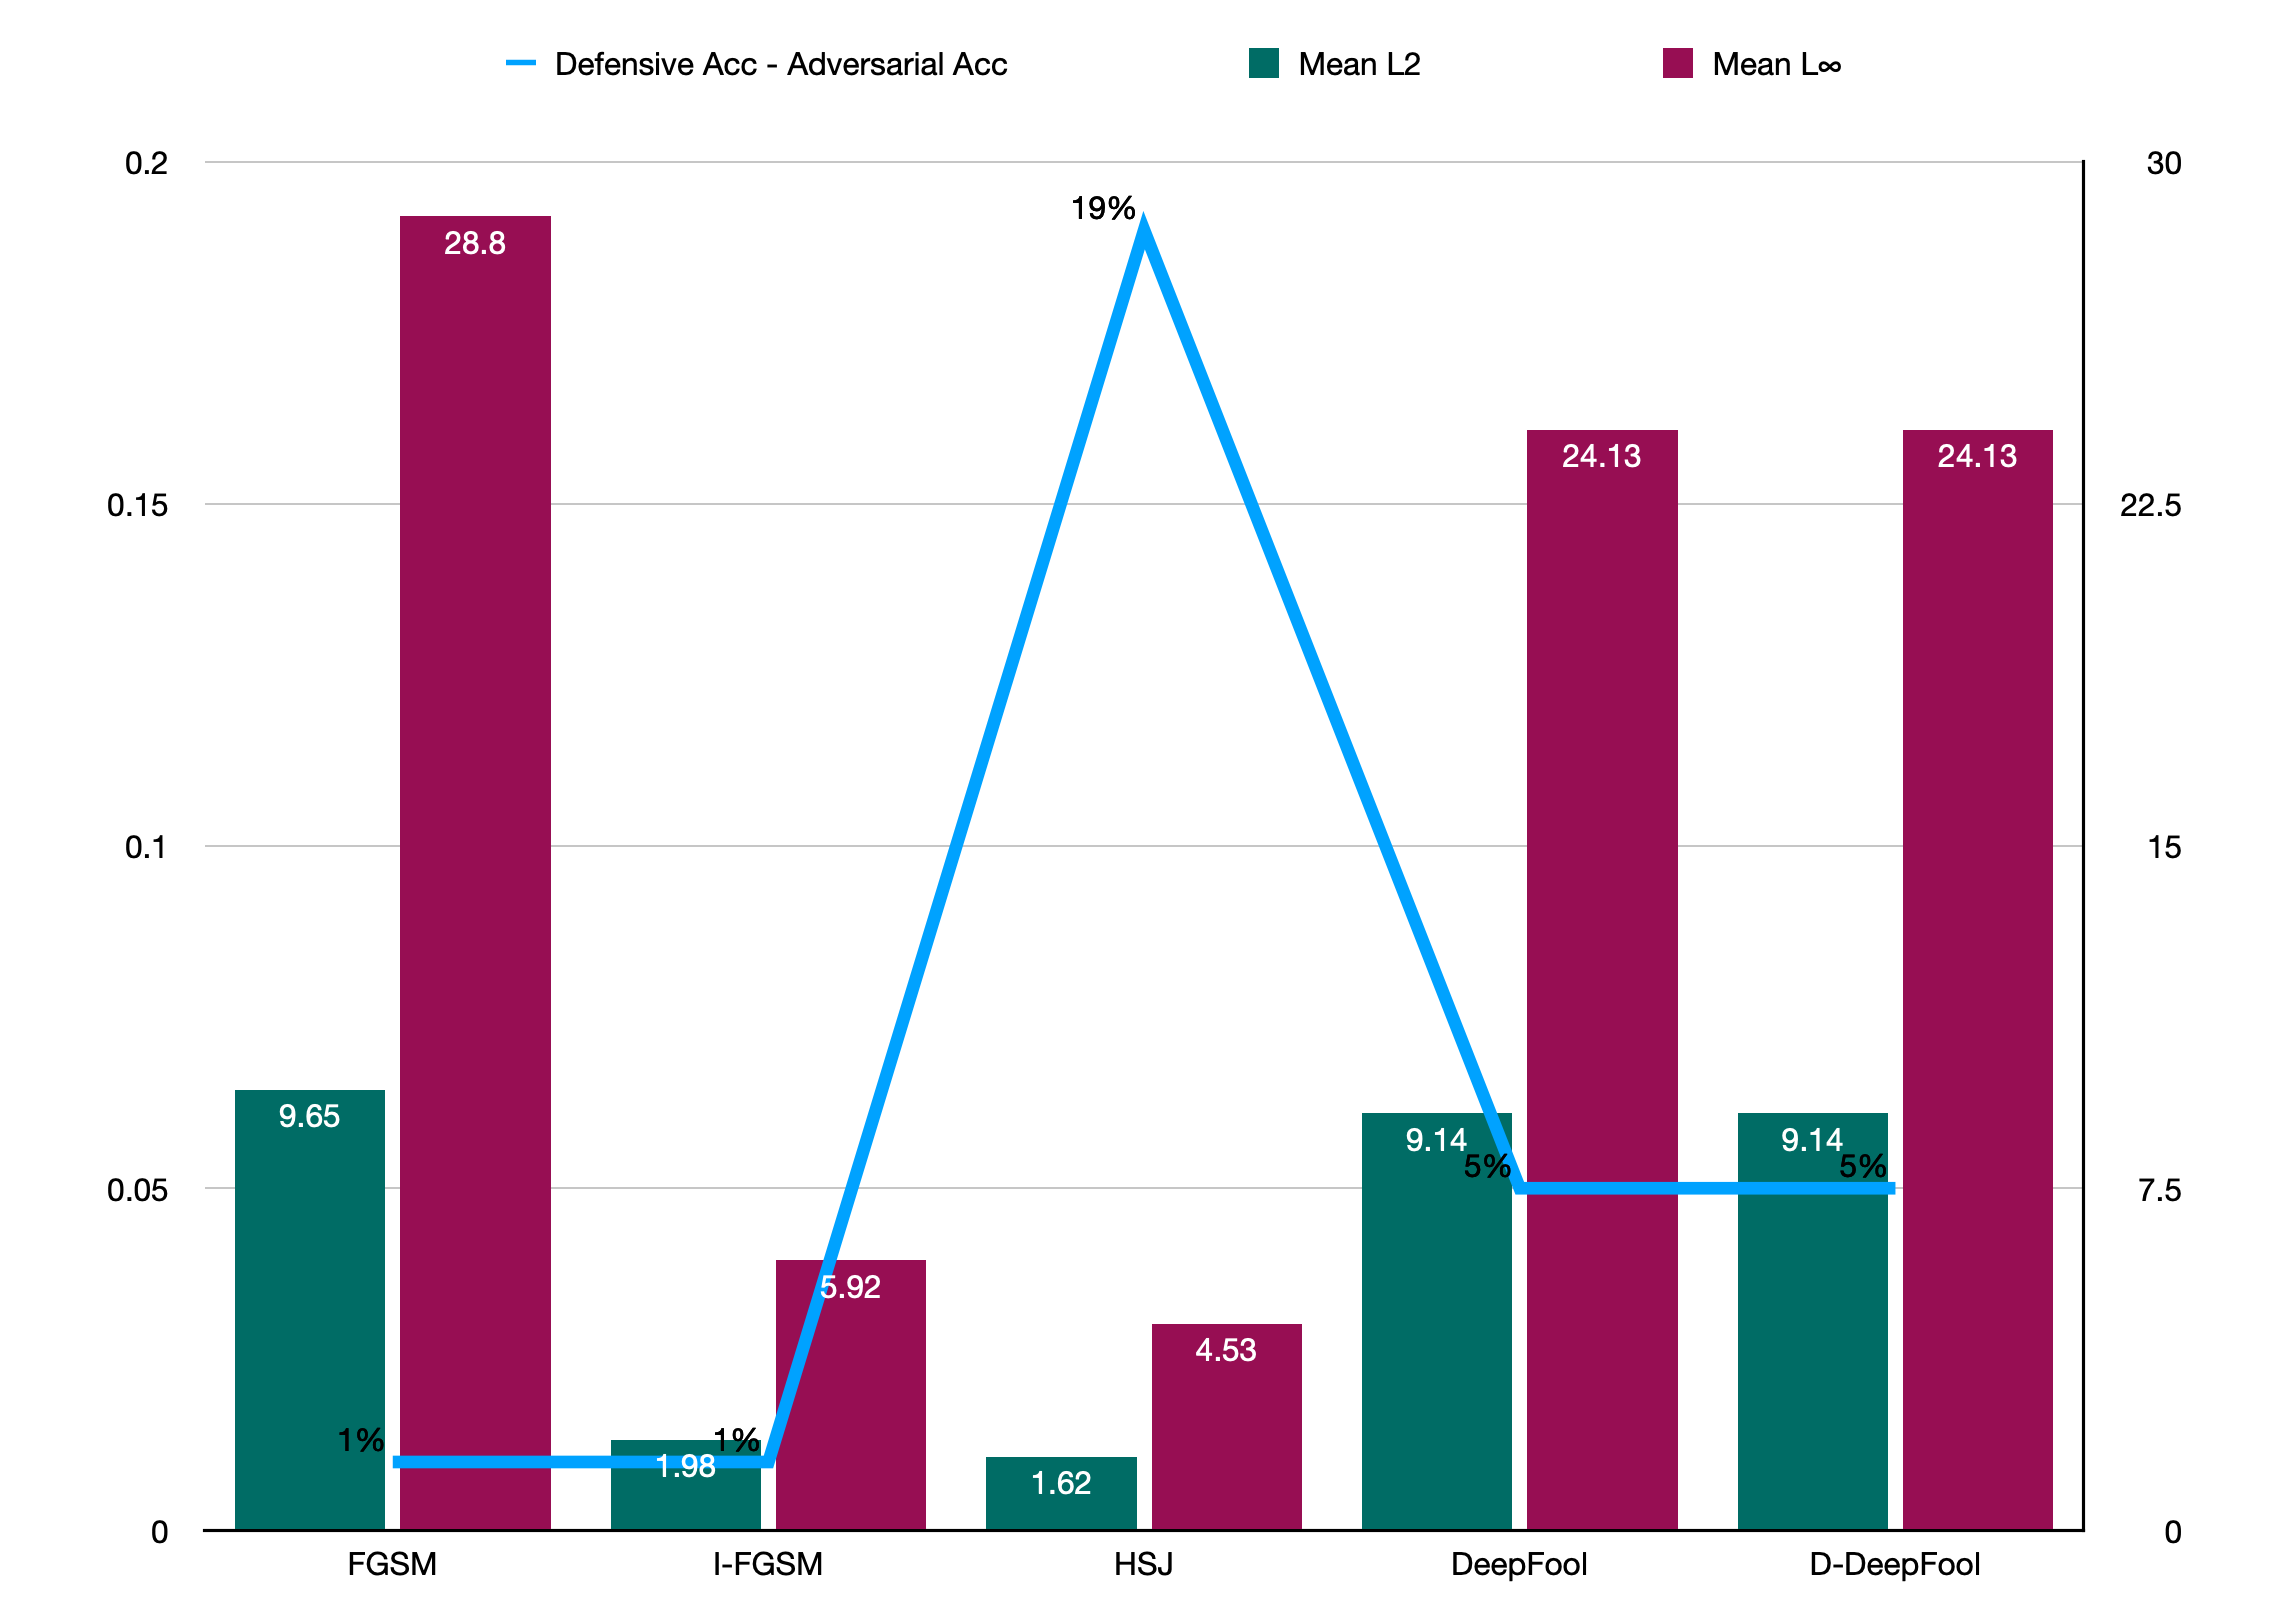
\includegraphics[width = 0.8\textwidth]{{fig/ss_cifar10_budget.png}}
    \caption{Budget comparision}
    \label{ss_cifar10_budget}
\endminipage
\caption*{Evasion attack algorithms v. \ilc{Spatial Smoothing} on \textit{CIFAR-10}}
\end{figure}


\ilc{Spatial Smoothing} a.k.a. \ilc{SS} is our implemented defense algorithm to increase model's robustness against adversarial input -- as it actually actually help predicting the true label of an adversarial image. We may proudly say that there is a $38 \%$ \textit{accuracy} before and after the \ilc{SS} being implemented across our four experimented algorithms (we exclude \ilc{D-DeepFool} for this disscussion as it performs identical to standard \ilc{DeepFool}) on \textit{MINIST}.

Note this experiment also confirms the fact that \ilc{HSJ} is probably not ``converged'' yet with its current setting on \textit{MINIST}, as it has again costed high \textit{perturbation budget}. We also observed the higher the \textit{pertubation budget}, the better the defensive effectiveness -- this is again in accordance with out intuition as we as human can also distinguish highly perturbed picture well.\newline

Also note  [\figurename{\ \ref{bd_minist_budget}}] seems to be suggesting low \textit{pertubation budget} will result in high model effectiveness, this is only semi-true as the overall effectiveness increase on \textit{CIFAR-10} is comparatively low (only $+6.5 \%$ among the $4$ experimented algorithms, where it is $+38 \%$ in \textit{MINIST}), so it is more of \ilc{SS} being effective against \ilc{HSJ}.

We believe this have something to do with the fact \ilc{SS} look into the activations of neuros of adversarial pattern and either force-zero or oppress them. As \ilc{HSJ} being on the decisions boundaries (implied by the low \textit{pertubation budget}), a \ilc{HSJ}-generated adversarial imag might be considered to have adversarial patterns of many kinds and therefore being detected by the defense algorithm.

Minyang, please correct me if I am wrong and add some insight.

\subsubsection{Transformer}\label{defense_transformer}

\begin{figure}[H]
    \centering
    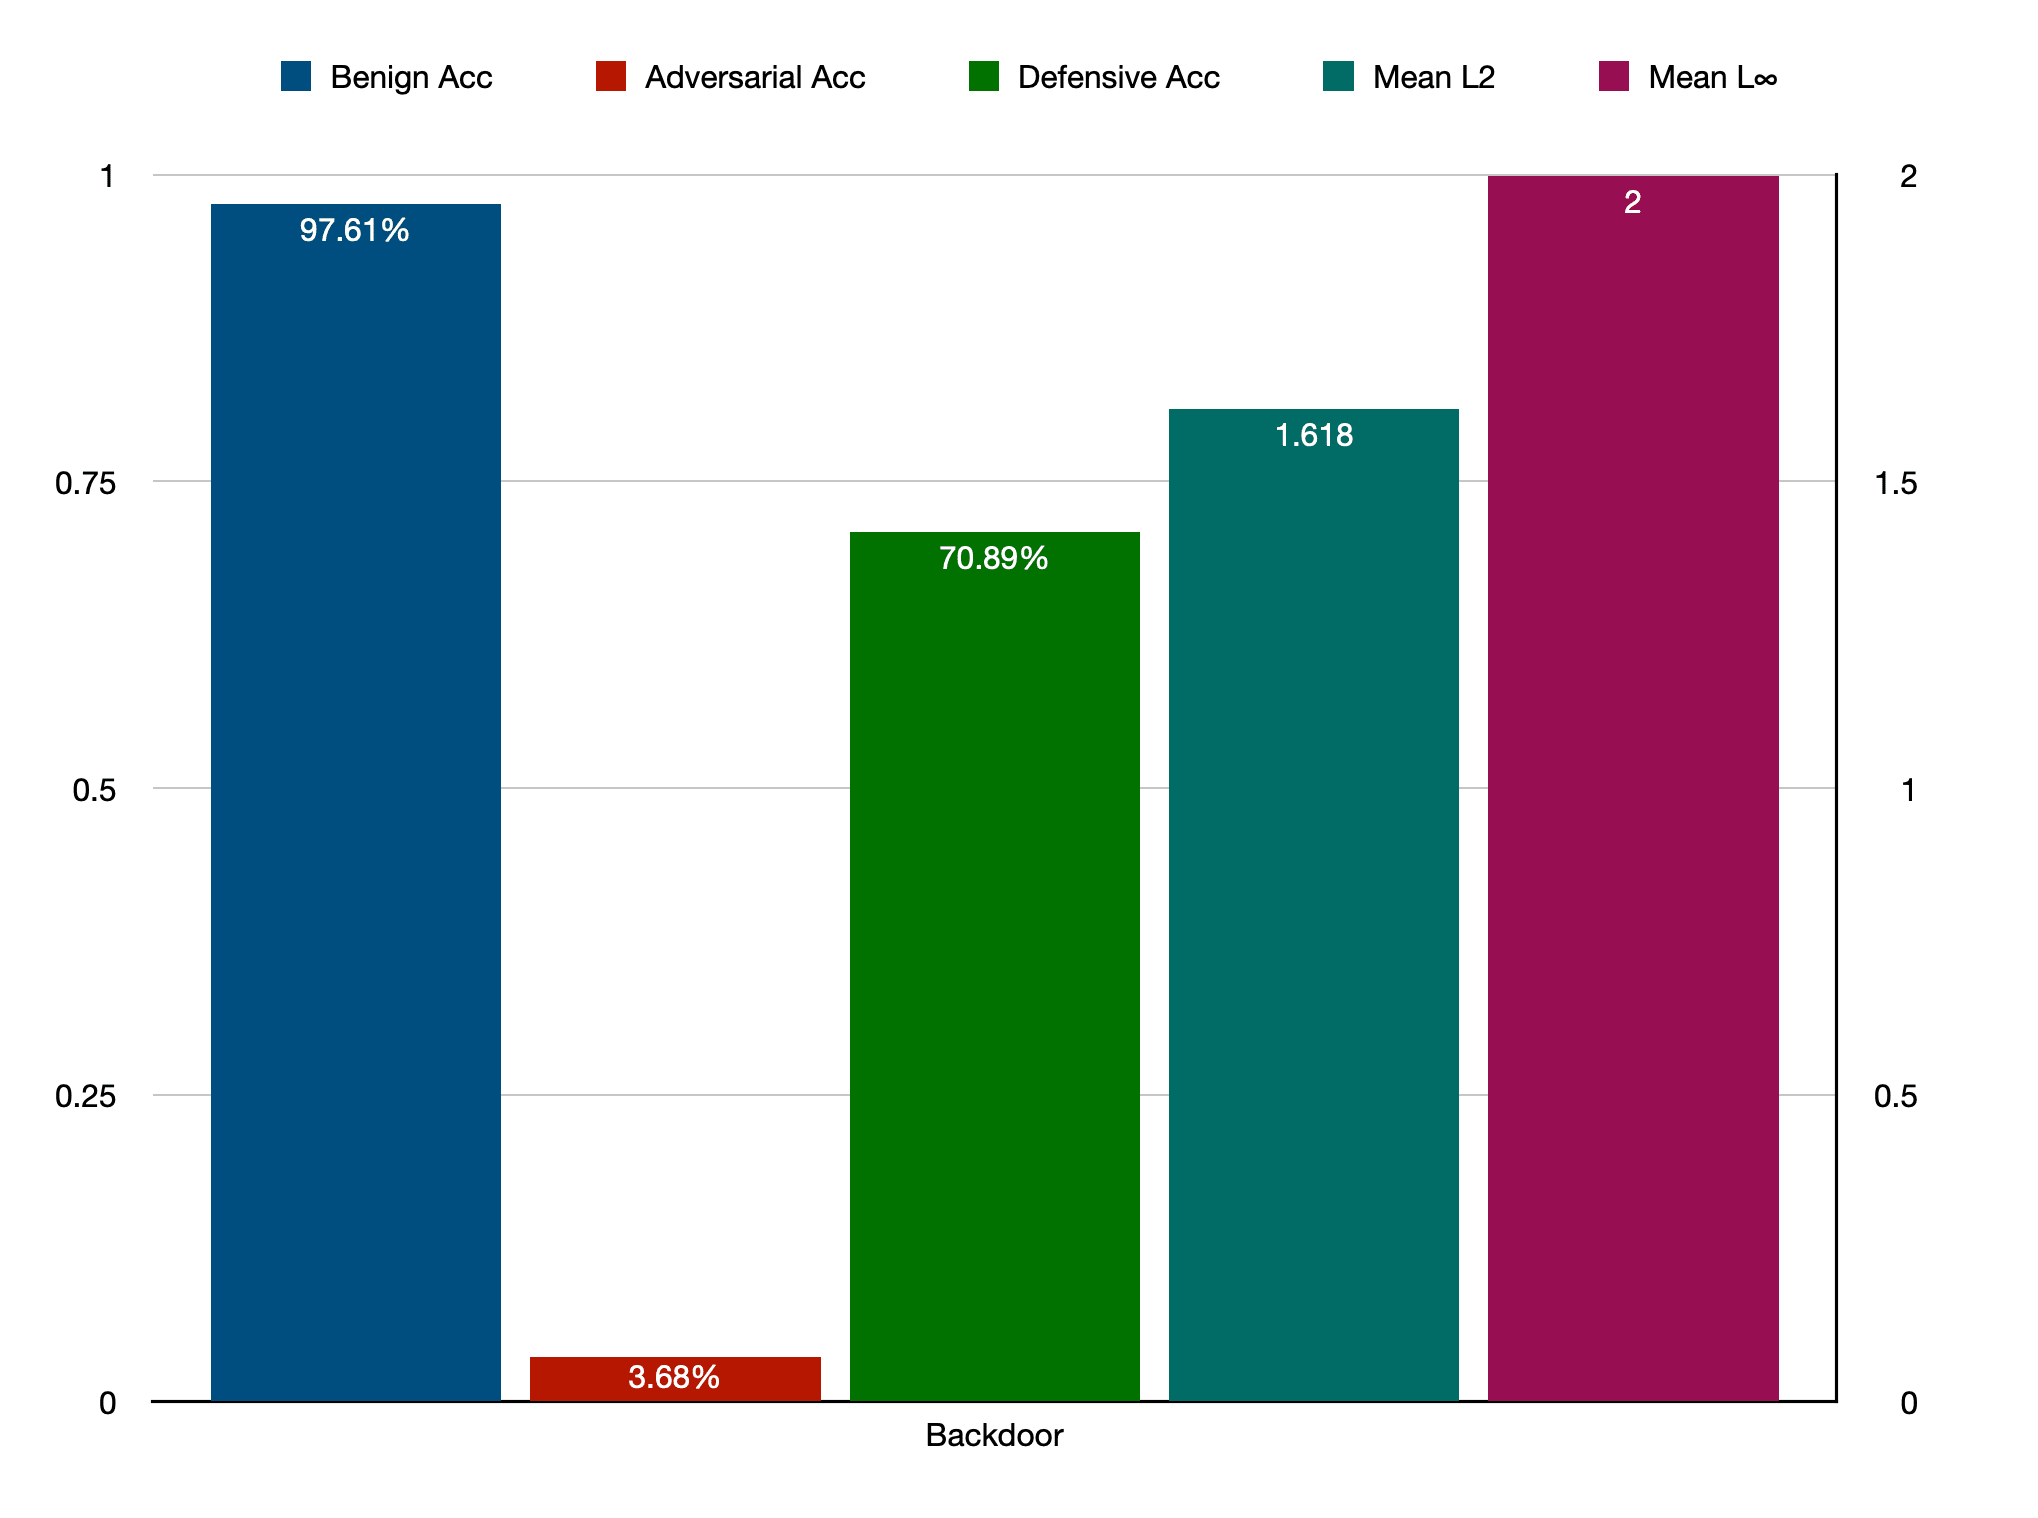
\includegraphics[width = 0.8\textwidth]{{fig/nc_backdoor_acc_budget.png}}
    \caption{\ilc{Backdoor} v. \ilc{Neural Cleanse}}
    \label{nc_backdoor_acc_budget}
\end{figure}

Minyang please explain why this works.

\subsubsection{Conclusion}

As each defensive algorithms have their different purposes and propertities, it is hard to conclude them generally. But base on our consistent observation, it might be safe to say an adversarial example with less \textit{budger pertubation} is likely likely to be detected by a defensive algorithm -- which is consistent to our intuition and the geometrical stucture of feature space and decision boundaries: as if something is the middle of several boundaries, it will be hard to distinguish wheather it is an adversarial example of just an ``outliner'' of a neighborhood class.

In a partical sense, it might be best

% % % % % % % % % % % % % % % % % % % % % % % % % % % % % % % % %
% % % % % % % % % % % % % % % % % % % % % % % % % % % % % % % % %
% % % % % % % % % % % % % % % % % % % % % % % % % % % % % % % % %
\section{References}
\nocite{*}
\raggedright
\bibliography{references.bib}
\bibliographystyle{plain}




\end{document}